% 1. Load tikz and pgfplots BEFORE the document class
\RequirePackage{tikz}
\RequirePackage{pgfplots}

% 2. Now define the document class
\documentclass{ieeeaccess}

% 3. Load the rest of your packages
\usepackage{cite}
\usepackage{amsmath,amssymb,amsfonts}
\usepackage{algorithmic}
\usepackage{graphicx}
\usepackage{textcomp}
\usepackage{placeins}
\usepackage{multirow}
\usepackage{colortbl}
\usepackage{xcolor}
\usepackage{booktabs}
\usepackage{array}


% 4. Load your tikz libraries and configurations normally
\usetikzlibrary{shapes.geometric, arrows, positioning, fit, backgrounds, calc, patterns, arrows.meta}
\pgfplotsset{compat=1.17}
\usepgfplotslibrary{statistics}

\def\BibTeX{{\rm B\kern-.05em{\sc i\kern-.025em b}\kern-.08em
    T\kern-.1667em\lower.7ex\hbox{E}\kern-.125emX}}

\begin{document}
\history{Date of publication xxxx 00, 0000, date of current version xxxx 00, 0000.}
\doi{10.1109/ACCESS.2017.DOI}

\title{Mechanistic LLM Control for ISO/IEC 29110 Compliance: A Structural Isomorphism Framework}

\author{\uppercase{Victor Terón-Macias}\authorrefmark{1},
\uppercase{Salvador Hinojosa\authorrefmark{1}, Miguel Gonzalez-Mendoza}.\authorrefmark{1}, and \uppercase{Jezreel Mejía \authorrefmark{2}} }
\address[1]{Tecnologico de Monterrey, Escuela de Ingeniería y Ciencias Boulder, Ave. Eugenio Garza Sada 2501 Sur, Col: Tecnológico, Monterrey, N.L., México, 64700. (e-mail: A00843371@tec.mx, salvador.hinojosa@tec.mx, mgonza@tec.mx)}
\address[2]{Centro de Investigación en Matemáticas Unidad Zacatecas, Departamento de Ingeniería de Software (e-mail: jmejia@cimat.mx)}

\tfootnote{This work was supported by the Tecnologico de Monterrey Campus Estado de México}

\markboth
{Terón-Macias \headeretal: Mechanistic LLM Control for ISO/IEC 29110 Compliance}
{Terón-Macias \headeretal: Mechanistic LLM Control for ISO/IEC 29110 Compliance}

\corresp{Corresponding author: Salvador Hinojosa (e-mail: salvador.hinojosa@tec.mx).}

\begin{abstract}
Compliance auditing of software engineering governance standards such as ISO/IEC 29110 in corporate repositories remains a manual, costly, and error-prone process. While Large Language Models (LLMs) offer the potential to automate such auditing, two fundamental barriers impede their empirical evaluation: (1) strict industrial privacy policies prevent the publication of corporate datasets, and (2) naive, uncalibrated LLMs produce unreliable classifications due to hallucinations and lack of normative grounding. This paper proposes a methodological framework based on structural isomorphism to generate privacy-preserving synthetic datasets, coupled with targeted mechanistic model enhancements to reduce unsupported or inconsistent classifications. We formalize a set of organizational meta-rules derived from ISO/IEC 29110 and synthesize a controlled environment (Biblio-VSE) constrained by \emph{partial structural isomorphism}: source-code complexity (McCabe's V(G)) satisfies both defined thresholds, but documentary Fog Index does not, so the benchmark approximates rather than fully replicates the reference corpus. Four open-weights foundation models (Gemma-2, Mistral, Qwen2.5, Phi-3.5) are evaluated across eight progressive configurations encompassing Zero-Shot prompting, Retrieval-Augmented Generation (RAG), and Activation Steering ($\alpha=0.8$). Retrieval-Augmented Generation over the ISO/IEC 29110 normative corpus (14 semantic chunks from \texttt{Metareglas extraidas.docx}) improves point estimates for all four models---Gemma-2 achieves F1=0.842 under Zero-Shot+RAG (Exp~5)---although no individual gain survives Holm--Bonferroni correction. Activation steering is the most consistently beneficial single intervention across all four architectures. The global maximum is F1=0.880 (95\,\% CI [0.70, 1.00]) for Phi-3.5-mini under Zero-Shot + Steering; pipeline gains are architecture-specific and Zero-Shot alone is destructive for Phi-3.5-mini ($\Delta$F1 $= -0.41$). \textbf{All F1 figures for steering-enhanced configurations should be treated as upper-bound estimates}: the intervention coefficient $\alpha=0.8$ was selected on the same 20 artifacts used for reporting, introducing in-sample optimism that cannot be corrected without a held-out validation split. Given the evaluation set of $N=20$ artifacts, all results are exploratory and hypothesis-generating rather than confirmatory. The proposed framework enables reproducible auditing of private repositories without compromising industrial trade secrets.
\end{abstract}

\begin{keywords}
Activation Steering, Artificial Intelligence, ISO/IEC 29110, Large Language Models, Software Standard Compliance, Structural Isomorphism, Synthetic Datasets.
\end{keywords}

\titlepgskip=-15pt

\maketitle


\section{Introduction}
\label{sec:introduction}

Very Small Entities (VSEs) play a significant role in software development ecosystems, but they often operate under severe resource constraints that limit their ability to adopt heavyweight process-assessment and governance frameworks. ISO/IEC 29110 was designed to address this context by defining lifecycle profiles for VSEs, including process guidance for project management and software implementation activities \cite{iso29110_2024,laporte2016vse,laporte2015implementation}. Empirical studies on ISO/IEC 29110 adoption show that the standard can support process improvement, organizational learning, communication, and traceability practices in small organizations, but they also report difficulties related to implementation effort, technical adoption, documentation, and sustained process execution \cite{munoz2020implementations,101145,claudiolapuerta}. These challenges are especially visible during compliance assessment and recertification, where organizations must provide documentary evidence showing that required work products, approvals, reviews, and traceability relationships have been properly established \cite{terronmacias,11276002}.

Traceability is one of the central governance mechanisms in ISO/IEC 29110 because it connects requirements, design elements, implementation artifacts, verification activities, test evidence, and approval records. Prior work on traceability recovery has shown that links between code and documentation can be recovered using information-retrieval techniques, and later systematic mappings have confirmed the importance of traceability-link recovery as a long-standing software engineering problem \cite{antoniol2002traceability,borg2013traceability}. More recent research has begun to explore retrieval-augmented generation and large language model (LLM) ensembles for traceability-link recovery and candidate filtering \cite{fuchss2025lissa,fuchss2025llmtrace}. Nevertheless, ISO/IEC 29110 compliance auditing differs from ordinary traceability recovery because the task is not only to identify artifact links, but also to decide whether those links, documents, reviews, and approvals satisfy normative process expectations defined by a standard \cite{iso29110_2024,castellanos2022processcompliance}.

The recent progress of LLMs has created new opportunities for automating software engineering tasks. Transformer-based and instruction-tuned models have demonstrated strong performance in code generation, code understanding, summarization, bug fixing, and benchmark-based software engineering evaluation \cite{jiang2024surveycodegen,lu2021codexglue,jimenez2023swebench,jain2024livecodebench}. Models such as CodeBERT, CodeT5, and StarCoder have advanced code-specific pretraining and code understanding capabilities \cite{feng2020codebert,wang2021codet5,li2023starcoder}. At the same time, open-weight general-purpose models such as LLaMA, Mistral, Phi, Gemma, and Qwen have expanded the feasibility of local and reproducible experimentation for software engineering tasks \cite{touvron2023llama,jiang2023mistral,abdin2024phi3,riviere2024gemma2,yang2024qwen25}. However, most of this progress has focused on functional correctness, programming ability, or code-level reasoning rather than governance-level compliance auditing.

Compliance auditing poses a different kind of challenge. Unlike code generation or issue resolution, compliance assessment requires the interpretation of heterogeneous documentary evidence, implicit organizational practices, traceability structures, and standard-defined obligations. Automated compliance checking has traditionally relied on rule-based, model-based, or formal approaches, including process-model compliance verification and formal representations of standard requirements \cite{castellanos2022processcompliance,castellanos2018spem,sirikrajai2025cpn,tuaycharoen2025auditorviews}. These approaches can provide precision when rules are explicit and artifacts are formally modeled, but they are less flexible when evidence appears in natural-language documents, informal repositories, review comments, approval logs, or partially structured traceability records. Semantic compliance-checking approaches attempt to address this gap by aligning natural-language rules and domain knowledge with compliance requirements \cite{guo2021semantic,zheng2022semantic}, yet systematic evaluation of LLMs as ISO/IEC 29110 governance auditors remains limited.

A second difficulty is the lack of privacy-preserving benchmarks for this type of evaluation. Industrial repositories contain proprietary source code, customer requirements, internal review discussions, project-management artifacts, and confidential approval evidence. Directly releasing such repositories for benchmark construction is therefore impractical. In the broader machine-learning literature, differential privacy and federated learning have been proposed as mechanisms for privacy-preserving learning \cite{dwork2006differentialprivacy,mcmahan2017communication}. In software engineering, synthetic data generation and synthetic software-engineering tasks have been proposed to reduce dependence on sensitive or unavailable data \cite{bauer2024syntheticdata,yang2025swesmith}. However, benchmark construction for compliance auditing requires more than generating plausible code or isolated tasks: the benchmark must preserve the structural topology of industrial repositories, including artifact dependencies, peer-review workflows, approval evidence, nonconformities, and traceability relations. This creates a need for synthetic repositories that are structurally isomorphic to real compliance environments while avoiding the disclosure of proprietary artifacts.

A third difficulty concerns the reliability of LLMs when used for strict classification and evaluation tasks. General studies of LLM evaluation show that model assessment remains difficult across tasks, benchmarks, and evaluation protocols \cite{asoeollm}. Recent work on LLM-as-a-judge in software engineering suggests that LLM evaluators can sometimes approximate human judgment, but their alignment with expert assessment depends on the task, scoring method, and evaluation design \cite{cllmrheaesllmis,ICLR2025_7f8f7313}. For normative compliance auditing, this limitation is critical because an incorrect judgment may cause an organization to overlook a missing approval, broken traceability link, or incomplete work product. Moreover, benchmark contamination and inter-dataset code duplication can distort LLM evaluation results in software engineering \cite{hernandez2024codeduplication,zhou2025lessleak}. These risks motivate evaluation designs that distinguish prompt-based behavior from more controlled model interventions.

Mechanistic interpretability and representation engineering offer a complementary direction. Prior work suggests that high-level behavioral concepts can be represented as directions in activation space and that manipulating these directions can alter model behavior during inference \cite{zou2023representation,turner2023activation}. Inference-time intervention has also been explored as a way to elicit more truthful answers from language models \cite{li2023iti}. Unlike prompt engineering, activation steering modifies internal model states rather than only adding external natural-language instructions. This property makes activation steering attractive for compliance auditing, where the model must remain sensitive to normative distinctions even when the input contains long, noisy, or conflicting documentary evidence. Nevertheless, the use of activation steering for ISO/IEC 29110 compliance evaluation has not been systematically investigated.

This article addresses these gaps by proposing a structural isomorphism framework for evaluating LLM-based ISO/IEC 29110 compliance auditing under privacy-preserving conditions. The framework constructs synthetic repositories that preserve the governance topology of industrial software projects while replacing proprietary content with non-sensitive artifacts. It then evaluates multiple LLM configurations, including zero-shot prompting, retrieval-augmented generation, rule-based baselines, and activation steering. The central hypothesis is that compliance auditing benefits not only from retrieving relevant artifacts, but also from steering internal model representations toward normative distinctions between compliant and non-compliant evidence. Figure~\ref{fig:conceptual_framework} summarizes the conceptual relationship among industrial compliance evidence, synthetic structural isomorphism, and LLM-based auditing.

\begin{figure}[!t]
\centering
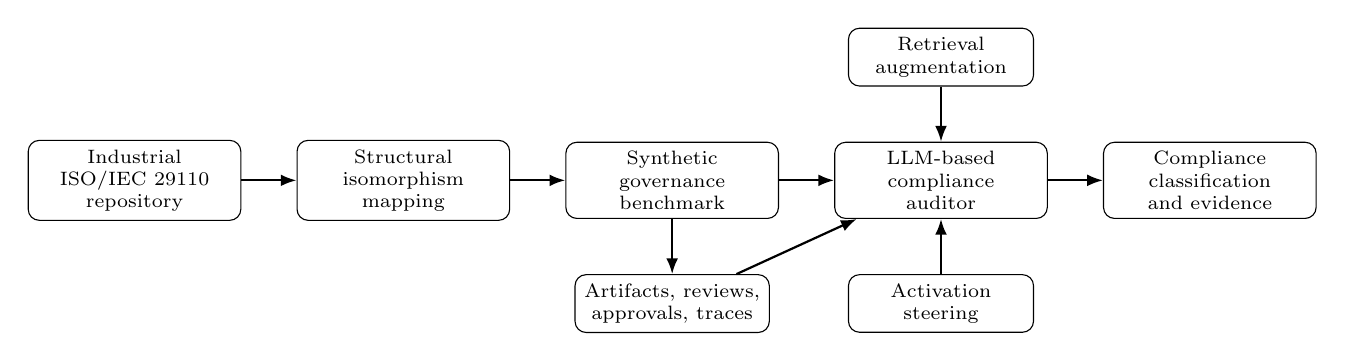
\begin{tikzpicture}[
    node distance=7mm and 7mm,
    block/.style={rectangle, rounded corners, draw, align=center, minimum width=2.7cm, minimum height=8mm, font=\scriptsize},
    smallblock/.style={rectangle, rounded corners, draw, align=center, minimum width=2.35cm, minimum height=7mm, font=\scriptsize},
    arrow/.style={-{Latex[length=2mm]}, thick}
]
\node[block] (industrial) {Industrial\\ISO/IEC 29110\\repository};
\node[block, right=of industrial] (isomorphism) {Structural\\isomorphism\\mapping};
\node[block, right=of isomorphism] (synthetic) {Synthetic\\governance\\benchmark};
\node[smallblock, below=of synthetic] (evidence) {Artifacts, reviews,\\approvals, traces};
\node[block, right=of synthetic] (llm) {LLM-based\\compliance\\auditor};
\node[smallblock, above=of llm] (rag) {Retrieval\\augmentation};
\node[smallblock, below=of llm] (steering) {Activation\\steering};
\node[block, right=of llm] (decision) {Compliance\\classification\\and evidence};

\draw[arrow] (industrial) -- (isomorphism);
\draw[arrow] (isomorphism) -- (synthetic);
\draw[arrow] (synthetic) -- (llm);
\draw[arrow] (llm) -- (decision);
\draw[arrow] (synthetic) -- (evidence);
\draw[arrow] (evidence) -- (llm);
\draw[arrow] (rag) -- (llm);
\draw[arrow] (steering) -- (llm);
\end{tikzpicture}
\caption{Conceptual framework linking ISO/IEC 29110 industrial repositories, privacy-preserving structural isomorphism, synthetic benchmark construction, and LLM-based compliance auditing.}
\label{fig:conceptual_framework}
\end{figure}

The contributions of this article are fourfold. First, it formalizes ISO/IEC 29110 compliance auditing as a normative classification problem over documentary artifacts, traceability relations, review evidence, and approval records \cite{iso29110_2024,terronmacias,11276002}. Second, it proposes a privacy-preserving synthetic benchmark construction strategy based on structural isomorphism rather than direct repository disclosure \cite{bauer2024syntheticdata,dwork2006differentialprivacy,mcmahan2017communication}. Third, it empirically compares rule-based checking, zero-shot LLM prompting, retrieval-augmented generation, and activation steering for compliance classification \cite{castellanos2022processcompliance,fuchss2025lissa,zou2023representation,turner2023activation}. Fourth, it analyzes the implications of mechanistic model intervention for software-process governance, especially in VSE contexts where manual audit effort and documentation overhead remain major barriers to standard adoption \cite{laporte2016vse,munoz2020implementations,101145}.

The remainder of this article is organized as follows. Section~\ref{sec:slr_methodology} describes the systematic literature review protocol used to identify and synthesize prior work. Section~\ref{sec:related_work} presents the related work derived from the review, organized around LLMs for software engineering, privacy-preserving benchmarking, activation steering, and automated compliance auditing. Section~\ref{sec:methodology} introduces the proposed structural isomorphism and activation-steering framework. Section~\ref{sec:setup} describes the experimental design, datasets, models, and baselines. Section~\ref{sec:results} reports the empirical results. Section~\ref{sec:discussion} discusses implications, limitations, and threats to validity. Section~\ref{sec:conclusion} concludes the article and outlines future research directions.

\section{Literature Selection Method}
\label{sec:slr_methodology}

This study followed a systematic literature review (SLR) protocol grounded in the evidence-based software engineering guidelines proposed by Kitchenham and Charters and later consolidated in tertiary studies of software engineering SLR practice \cite{kitchenham2007guidelines,kitchenham2010tertiary}. Because the topic spans software engineering benchmarks, ISO/IEC 29110 compliance, traceability, LLM evaluation, synthetic data, and mechanistic model intervention, the protocol combined database search with snowballing. This hybrid strategy was selected because database search and snowballing have been shown to retrieve complementary bodies of software engineering literature \cite{jalali2012database,wohlin2014snowballing,wohlin2022hybrid}. Figure~\ref{fig:slr_protocol} summarizes the review process.

\begin{figure}[!t]
\centering
\begin{tikzpicture}[
    node distance=6mm,
    step/.style={rectangle, rounded corners, draw, align=center, minimum width=6.5cm, minimum height=7mm, font=\scriptsize},
    decision/.style={diamond, draw, align=center, aspect=2.2, inner sep=1pt, font=\scriptsize},
    arrow/.style={-{Latex[length=2mm]}, thick}
]
\node[step] (protocol) {Define review protocol\\research questions, scope, criteria};
\node[step, below=of protocol] (search) {Database search\\IEEE Xplore, ACM DL, Scopus, SpringerLink, ScienceDirect, arXiv};
\node[step, below=of search] (dedup) {Deduplicate records\\remove repeated and non-scholarly entries};
\node[step, below=of dedup] (screen) {Title, abstract, and keyword screening};
\node[step, below=of screen] (fulltext) {Full-text eligibility assessment};
\node[step, below=of fulltext] (snowball) {Backward and forward snowballing};
\node[step, below=of snowball] (extract) {Data extraction and quality assessment};
\node[step, below=of extract] (synthesis) {Thematic synthesis\\related work and research gap};

\draw[arrow] (protocol) -- (search);
\draw[arrow] (search) -- (dedup);
\draw[arrow] (dedup) -- (screen);
\draw[arrow] (screen) -- (fulltext);
\draw[arrow] (fulltext) -- (snowball);
\draw[arrow] (snowball) -- (extract);
\draw[arrow] (extract) -- (synthesis);
\end{tikzpicture}
\caption{Systematic literature review protocol combining Kitchenham-style evidence-based software engineering guidelines with Wohlin-style snowballing \cite{kitchenham2007guidelines,kitchenham2010tertiary,wohlin2014snowballing,wohlin2022hybrid}.}
\label{fig:slr_protocol}
\end{figure}

\subsection{Review Objectives and Research Questions}
\label{subsec:slr_rqs}

The objective of the SLR was to identify the bodies of literature required to position this work at the intersection of ISO/IEC 29110 compliance auditing, software engineering benchmarks, privacy-preserving synthetic data, LLM-based software engineering, and activation steering. The review was organized around the following research questions:

\begin{itemize}
    \item \textbf{RQ1:} How have LLMs been evaluated for software engineering tasks, and what limitations remain for governance-level assessment?
    \item \textbf{RQ2:} What approaches have been proposed for privacy-preserving or synthetic benchmark construction in software engineering and machine learning?
    \item \textbf{RQ3:} How have mechanistic interpretability, representation engineering, and activation steering been used to control or modify LLM behavior?
    \item \textbf{RQ4:} What methods exist for automated compliance checking, requirements traceability, and ISO/IEC 29110 assessment?
    \item \textbf{RQ5:} What research gap emerges when these areas are considered together?
\end{itemize}

These research questions were designed to support both the methodological contribution and the empirical evaluation of the article. RQ1 identifies the capabilities and limitations of current LLMs for software engineering \cite{jiang2024surveycodegen,lu2021codexglue,jimenez2023swebench,jain2024livecodebench}. RQ2 addresses the privacy and benchmark-construction problem \cite{bauer2024syntheticdata,yang2025swesmith,hernandez2024codeduplication,zhou2025lessleak}. RQ3 establishes the basis for activation steering as a model-intervention technique \cite{zou2023representation,turner2023activation,li2023iti}. RQ4 connects compliance auditing to ISO/IEC 29110, traceability, and automated compliance checking \cite{iso29110_2024,laporte2016vse,castellanos2022processcompliance,antoniol2002traceability,borg2013traceability}. RQ5 synthesizes these strands into the research gap addressed by this article.

\subsection{Search Strategy}
\label{subsec:slr_search_strategy}

The search strategy combined automated database queries with targeted snowballing. The database search covered major digital libraries relevant to software engineering, artificial intelligence, and standards-oriented research, including IEEE Xplore, ACM Digital Library, Scopus, SpringerLink, ScienceDirect, and arXiv. Search strings were constructed from five concept groups: LLMs for software engineering, software engineering benchmarks, synthetic or privacy-preserving data, activation steering or representation engineering, and compliance auditing or ISO/IEC 29110. The general form of the search string was:

\begin{quote}
\small
(\texttt{``large language model''} OR \texttt{LLM} OR \texttt{code model} OR \texttt{software engineering agent}) AND
(\texttt{benchmark} OR \texttt{evaluation} OR \texttt{traceability} OR \texttt{compliance}) AND
(\texttt{synthetic data} OR \texttt{privacy-preserving} OR \texttt{activation steering} OR \texttt{representation engineering} OR \texttt{ISO/IEC 29110})
\end{quote}

Because overly broad search strings can omit domain-specific terminology, additional targeted searches were executed for each thematic area. For LLMs and code analysis, the search emphasized code generation, code understanding, and software engineering benchmarks \cite{jiang2024surveycodegen,lu2021codexglue,feng2020codebert,wang2021codet5,li2023starcoder}. For privacy-preserving benchmarking, the search emphasized synthetic data, benchmark leakage, differential privacy, and federated learning \cite{bauer2024syntheticdata,dwork2006differentialprivacy,mcmahan2017communication,hernandez2024codeduplication,zhou2025lessleak}. For activation steering, the search emphasized representation engineering, activation engineering, and inference-time intervention \cite{zou2023representation,turner2023activation,li2023iti}. For compliance auditing, the search emphasized ISO/IEC 29110, process compliance, traceability, formal verification, semantic rule checking, and VSE adoption \cite{iso29110_2024,laporte2016vse,castellanos2022processcompliance,sirikrajai2025cpn,tuaycharoen2025auditorviews}.

\subsection{Inclusion and Exclusion Criteria}
\label{subsec:slr_criteria}

Inclusion and exclusion criteria were defined before full-text screening to reduce selection bias, following established SLR practice in software engineering \cite{kitchenham2007guidelines,kitchenham2010tertiary}. A study was included if it satisfied at least one of the following conditions:

\begin{itemize}
    \item It proposed, evaluated, or surveyed LLMs for software engineering, code understanding, code generation, or software engineering benchmarks.
    \item It addressed privacy-preserving data generation, synthetic data, benchmark leakage, or data contamination in machine learning or software engineering evaluation.
    \item It introduced or empirically evaluated activation steering, representation engineering, inference-time intervention, or related mechanistic model-control techniques.
    \item It addressed ISO/IEC 29110 adoption, VSE process improvement, traceability records, process compliance, automated compliance checking, or semantic rule interpretation.
    \item It provided methodological guidance for SLRs, software engineering evidence synthesis, or snowballing.
\end{itemize}

A study was excluded if it was not peer reviewed and did not provide technical detail, if it was unrelated to software engineering, compliance, benchmarking, or model intervention, if it discussed AI governance only at a high policy level without implications for evaluation or compliance, or if it lacked sufficient methodological information to support synthesis. Preprints were retained when they represented influential or technically relevant work not yet superseded by archival versions, which is common in rapidly developing LLM research \cite{touvron2023llama,jiang2023mistral,abdin2024phi3,riviere2024gemma2,yang2024qwen25}.

\subsection{Snowballing Procedure}
\label{subsec:slr_snowballing}

After the initial database search and full-text screening, backward and forward snowballing were performed following Wohlin's guidelines \cite{wohlin2014snowballing}. Backward snowballing inspected the reference lists of selected seed papers to identify earlier foundational work. Forward snowballing identified later studies that cited the seed papers. This procedure was particularly important for three reasons. First, LLM evaluation and activation steering are fast-moving research areas where influential work may appear first as preprints. Second, ISO/IEC 29110 research is distributed across standards literature, software process improvement, VSE case studies, traceability research, and formal compliance checking. Third, compliance auditing draws from adjacent domains such as semantic rule checking and automated regulatory compliance \cite{guo2021semantic,zheng2022semantic}. The snowballing process therefore reduced the risk of missing relevant studies that would not be captured by a single database query \cite{jalali2012database,wohlin2022hybrid}.

\begin{figure}[!t]
\centering
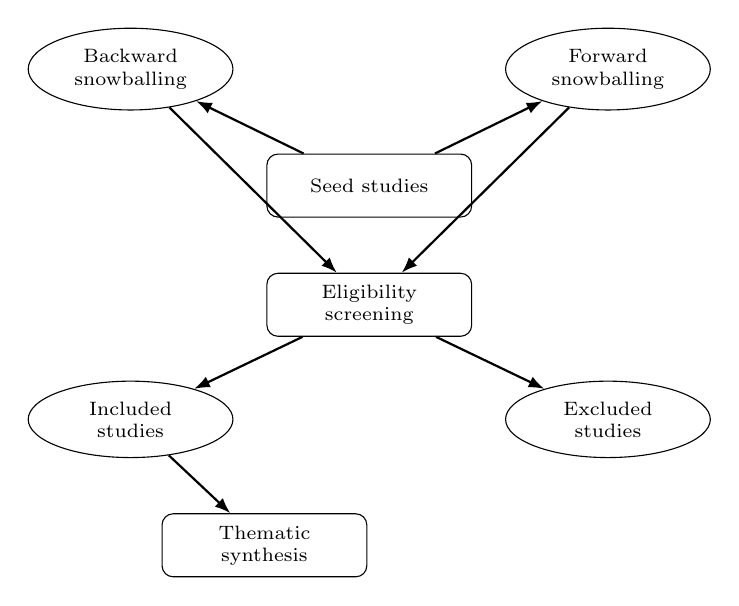
\begin{tikzpicture}[
    node distance=7mm and 8mm,
    seed/.style={rectangle, rounded corners, draw, align=center, minimum width=2.6cm, minimum height=8mm, font=\scriptsize},
    topic/.style={ellipse, draw, align=center, minimum width=2.6cm, minimum height=8mm, font=\scriptsize},
    arrow/.style={-{Latex[length=2mm]}, thick}
]
\node[seed] (seed) {Seed studies};
\node[topic, above left=of seed] (back) {Backward\\snowballing};
\node[topic, above right=of seed] (forward) {Forward\\snowballing};
\node[seed, below=of seed] (screen) {Eligibility\\screening};
\node[topic, below left=of screen] (include) {Included\\studies};
\node[topic, below right=of screen] (exclude) {Excluded\\studies};
\node[seed, below=of include, xshift=1.7cm] (synthesis) {Thematic\\synthesis};

\draw[arrow] (seed) -- (back);
\draw[arrow] (seed) -- (forward);
\draw[arrow] (back) -- (screen);
\draw[arrow] (forward) -- (screen);
\draw[arrow] (screen) -- (include);
\draw[arrow] (screen) -- (exclude);
\draw[arrow] (include) -- (synthesis);
\end{tikzpicture}
\caption{Snowballing process used to extend the initial database search with backward and forward citation traversal \cite{jalali2012database,wohlin2014snowballing,wohlin2022hybrid}.}
\label{fig:snowballing_process}
\end{figure}

\subsection{Data Extraction and Thematic Synthesis}
\label{subsec:slr_data_extraction}

For each included study, the data extraction form captured the publication type, research objective, application domain, evaluation target, benchmark or dataset, model or method, compliance or traceability focus, privacy mechanism, and reported limitations. The extracted studies were then coded into five themes: LLMs for software engineering, privacy-preserving benchmarking and synthetic data, mechanistic interpretability and activation steering, automated compliance auditing and ISO/IEC 29110, and requirements traceability. The coding process enabled a thematic synthesis that connects otherwise separate research areas. Table~\ref{tab:slr_themes} summarizes the role of each theme in the article.

\begin{table}[!t]
\centering
\caption{Themes identified through the SLR and their role in this article}
\label{tab:slr_themes}
\scriptsize
\begin{tabular}{p{0.22\linewidth} p{0.34\linewidth} p{0.34\linewidth}}
\toprule
\textbf{Theme} & \textbf{Representative literature} & \textbf{Role in this article} \\
\midrule
LLMs for software engineering & Code models, code benchmarks, SE agents, LLM evaluation \cite{jiang2024surveycodegen,lu2021codexglue,jimenez2023swebench,jain2024livecodebench} & Establishes the technical feasibility and limitations of LLM-based software engineering automation. \\
Synthetic and privacy-preserving benchmarks & Synthetic data, data leakage, differential privacy, federated learning \cite{bauer2024syntheticdata,yang2025swesmith,hernandez2024codeduplication,zhou2025lessleak,dwork2006differentialprivacy,mcmahan2017communication} & Motivates structurally isomorphic synthetic repositories for privacy-preserving compliance evaluation. \\
Activation steering & Representation engineering, activation engineering, inference-time intervention \cite{zou2023representation,turner2023activation,li2023iti} & Provides the basis for testing mechanistic intervention in normative compliance classification. \\
Compliance auditing and ISO/IEC 29110 & VSE standards, process compliance, formal verification, auditor views \cite{iso29110_2024,laporte2016vse,castellanos2022processcompliance,sirikrajai2025cpn,tuaycharoen2025auditorviews} & Defines the normative target of the proposed auditing framework. \\
Traceability recovery & Classical IR traceability, systematic mappings, RAG-based traceability \cite{antoniol2002traceability,borg2013traceability,fuchss2025lissa,fuchss2025llmtrace} & Provides the artifact-linking foundation required for compliance evidence assessment. \\
\bottomrule
\end{tabular}
\end{table}

\section{Related Work}
\label{sec:related_work}

\subsection{LLMs for Software Engineering and Code Analysis}
\label{subsec:rw_llms_se}

The application of LLMs to software engineering has expanded rapidly from code completion and generation to broader tasks such as code understanding, summarization, repair, issue resolution, and repository-level automation. CodeXGLUE provided an early benchmark suite for code understanding and generation tasks, while later benchmarks such as SWE-bench and LiveCodeBench evaluated LLM behavior on real-world software issues and contamination-aware coding tasks \cite{lu2021codexglue,jimenez2023swebench,jain2024livecodebench}. Survey literature confirms that LLMs have become central to contemporary code-generation research and software engineering automation \cite{jiang2024surveycodegen}.

Code-specialized pretraining has been one important line of progress. CodeBERT introduced a bimodal pretraining approach for programming and natural languages, CodeT5 proposed identifier-aware encoder-decoder modeling, and StarCoder demonstrated the value of large-scale code-focused pretraining for open code generation models \cite{feng2020codebert,wang2021codet5,li2023starcoder}. In parallel, general-purpose open-weight models such as LLaMA, Mistral, Phi, Gemma, and Qwen have shown that instruction-tuned LLMs can perform competitively across many software engineering tasks without architectures designed exclusively for code \cite{touvron2023llama,jiang2023mistral,abdin2024phi3,riviere2024gemma2,yang2024qwen25}.

Despite this progress, the dominant evaluation focus remains functional correctness, benchmark performance, or output quality. These objectives differ from governance-level compliance auditing, where the model must evaluate whether documentary evidence satisfies process obligations defined by a standard. LLM evaluation research also shows that model assessment is itself a difficult problem, especially when LLMs are used as judges or when benchmark contamination affects measured performance \cite{asoeollm,cllmrheaesllmis,ICLR2025_7f8f7313,hernandez2024codeduplication,zhou2025lessleak}. Therefore, evidence from code-generation benchmarks cannot be directly assumed to transfer to ISO/IEC 29110 compliance classification.

\subsection{Privacy-Preserving Benchmarking and Synthetic Data}
\label{subsec:rw_privacy_synthetic}

The construction of public benchmarks for industrial software engineering is constrained by privacy, intellectual property, and confidentiality. Real repositories may contain proprietary code, customer requirements, internal design decisions, personal data, security information, or commercially sensitive review discussions. Synthetic data generation has therefore become an important strategy for creating evaluation corpora without exposing private source material \cite{bauer2024syntheticdata}. In software engineering, synthetic task generation has also been explored as a mechanism for scaling agent evaluation and controlling benchmark properties \cite{yang2025swesmith}.

However, synthetic compliance benchmarks require a different design criterion from ordinary synthetic code datasets. A benchmark for ISO/IEC 29110 auditing must preserve not only realistic source-code structure, but also documentary topology: requirements specifications, project plans, meeting records, test cases, verification evidence, traceability matrices, review logs, approval records, and nonconformity patterns. The challenge is therefore structural as much as textual. The benchmark must retain the compliance-relevant relationships among artifacts while replacing private content with safe synthetic equivalents.

Privacy-preserving machine learning methods such as differential privacy and federated learning address related but distinct problems. Differential privacy provides mathematical guarantees that individual data contributions are protected during analysis or learning \cite{dwork2006differentialprivacy}. Federated learning enables model training across decentralized data without centralizing raw datasets \cite{mcmahan2017communication}. These approaches are important for privacy-preserving model training, but they do not directly solve the benchmark-publication problem addressed in this article. The present work instead focuses on privacy-preserving benchmark construction through structural isomorphism: the synthetic benchmark is designed to preserve governance relationships without disclosing the original repository.

Benchmark contamination and data leakage further complicate software engineering evaluation. Studies on inter-dataset code duplication and benchmark leakage show that LLM performance can be distorted when evaluation data overlaps with training data or with other public benchmarks \cite{hernandez2024codeduplication,zhou2025lessleak}. These findings strengthen the case for controlled benchmark construction, explicit artifact provenance, and synthetic repositories whose compliance labels are generated from known structural rules rather than from ambiguous public code corpora.

\subsection{Mechanistic Interpretability and Activation Steering}
\label{subsec:rw_activation_steering}

Mechanistic interpretability seeks to understand how neural networks represent and process information internally. Representation engineering extends this objective by treating high-level concepts as directions or structures in activation space that can be identified, analyzed, and manipulated \cite{zou2023representation}. Activation steering operationalizes this idea by modifying model activations during inference, often by adding a learned direction to internal residual-stream representations \cite{turner2023activation}. Related inference-time intervention methods have shown that internal activations can be manipulated to influence truthfulness and other behavioral properties of LLM outputs \cite{li2023iti}.

Most activation-steering studies focus on general behavioral dimensions such as truthfulness, sentiment, refusal behavior, toxicity, or broad preference alignment. Compliance auditing differs from these settings because the target behavior is domain-specific and normative. The desired distinction is not simply whether an answer is positive, safe, or truthful, but whether the model can classify documentary evidence according to a formal standard. This requires the model to attend to artifact completeness, traceability relations, review evidence, approval status, and the absence or presence of required work products.

Activation steering is relevant to this problem because prompt-only methods may fail when the context contains long documents, partial evidence, or conflicting signals. If compliance-relevant distinctions are represented in internal activation space, then steering vectors derived from compliant and non-compliant examples may improve classification consistency. This article therefore evaluates activation steering as a mechanistic intervention for ISO/IEC 29110 compliance classification, extending prior work on representation engineering and inference-time model control \cite{zou2023representation,turner2023activation,li2023iti}.

\subsection{Automated Compliance Auditing and ISO/IEC 29110}
\label{subsec:rw_compliance_iso}

ISO/IEC 29110 defines lifecycle profiles for VSEs and provides guidance intended to make systems and software engineering standards more accessible to small organizations \cite{iso29110_2024,laporte2016vse}. Studies of ISO/IEC 29110 implementation show that deployment packages, guides, and support tools can reduce adoption barriers, but they also indicate that organizations require practical support for documentation, traceability, and process institutionalization \cite{laporte2015implementation,munoz2020implementations,claudiolapuerta,101145}. Prior case-study work on traceability records further shows that ISO/IEC 29110 assessment can reveal incomplete coverage, missing traceability characteristics, and improvement needs during recertification \cite{terronmacias}.

Automated compliance checking has been studied in broader software-process and regulatory contexts. Systematic reviews show that compliance-checking approaches often rely on formalized process models, rule-based verification, or model-driven representations \cite{castellanos2022processcompliance}. Work using SPEM 2.0 process models and Colored Petri Nets illustrates how formal models can support compliance verification against safety or process standards \cite{castellanos2018spem,sirikrajai2025cpn,tuaycharoen2025auditorviews}. These methods are valuable when the relevant processes are explicitly represented, but they may be less effective when evidence is distributed across semi-structured repositories and natural-language artifacts.

Semantic compliance checking attempts to bridge formal rules and textual evidence by using domain knowledge, semantic alignment, and rule interpretation \cite{guo2021semantic,zheng2022semantic}. In software engineering, traceability recovery provides an adjacent foundation because compliance decisions often depend on whether required links exist among requirements, design elements, implementation artifacts, and test evidence \cite{antoniol2002traceability,borg2013traceability}. Recent LLM-based traceability research further suggests that retrieval-augmented generation and LLM ensembles can support traceability-link recovery and candidate filtering \cite{fuchss2025lissa,fuchss2025llmtrace}. However, traceability recovery alone does not decide whether a project satisfies ISO/IEC 29110 governance requirements. Compliance auditing requires the integration of traceability, document completeness, approval evidence, and standard-specific normative rules.

\subsection{Research Gap}
\label{subsec:rw_gap}

The reviewed literature reveals a convergence of three unresolved challenges. First, software engineering LLM research has produced strong evidence of model capability in code generation, code understanding, and benchmark-based task solving, but it has not systematically addressed governance-level compliance auditing \cite{jiang2024surveycodegen,lu2021codexglue,jimenez2023swebench,jain2024livecodebench}. Second, privacy-preserving and synthetic-data research provides mechanisms for reducing exposure of sensitive data, but existing approaches do not specifically preserve the governance topology required for ISO/IEC 29110 compliance evaluation \cite{bauer2024syntheticdata,dwork2006differentialprivacy,mcmahan2017communication,yang2025swesmith}. Third, activation steering has shown promise for controlling model behavior through internal representations, but its use for domain-specific normative classification remains underexplored \cite{zou2023representation,turner2023activation,li2023iti}.

This article addresses the gap by combining structural isomorphism, synthetic repository generation, and activation steering into a unified framework for ISO/IEC 29110 compliance auditing. The approach differs from prior traceability recovery because it evaluates compliance decisions rather than only artifact links. It differs from rule-based compliance checking because it evaluates natural-language and semi-structured evidence rather than only formal process models. It differs from ordinary LLM software engineering benchmarks because the target task is normative and governance-oriented rather than purely functional. Finally, it differs from generic synthetic data generation because the preservation target is not textual realism alone, but the compliance-relevant structure of an industrial repository.

\begin{figure}[!t]
\centering
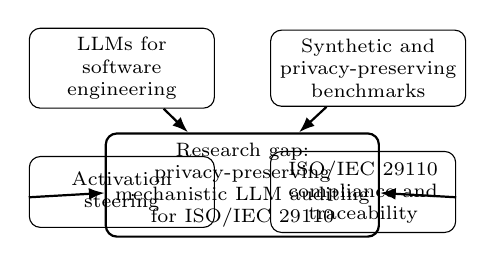
\begin{tikzpicture}[
    node distance=6mm and 7mm,
    area/.style={rectangle, rounded corners, draw, align=center, minimum width=2.35cm, minimum height=9mm, font=\scriptsize},
    center/.style={rectangle, rounded corners, draw, thick, align=center, minimum width=3.1cm, minimum height=12mm, font=\scriptsize},
    arrow/.style={-{Latex[length=2mm]}, thick}
]
\node[area] (llm) {LLMs for\\software\\engineering};
\node[area, right=of llm] (privacy) {Synthetic and\\privacy-preserving\\benchmarks};
\node[area, below=of llm] (steering) {Activation\\steering};
\node[area, right=of steering] (compliance) {ISO/IEC 29110\\compliance and\\traceability};
\node[center, below right=3mm and -14mm of llm] (gap) {Research gap:\\privacy-preserving\\mechanistic LLM auditing\\for ISO/IEC 29110};

\draw[arrow] (llm) -- (gap);
\draw[arrow] (privacy) -- (gap);
\draw[arrow] (steering) -- (gap);
\draw[arrow] (compliance) -- (gap);
\end{tikzpicture}
\caption{Positioning of the proposed work at the intersection of LLM-based software engineering, privacy-preserving benchmark construction, activation steering, and ISO/IEC 29110 compliance auditing.}
\label{fig:research_gap}
\end{figure}




\section{Methodology}
\label{sec:methodology}

\subsection{Problem Formalization and Meta-Rule Derivation}
\label{sec:formalization}

The ISO/IEC 29110 standard defines a basic profile for Very Small Entities (VSEs) structured into Project Management (PM) and Software Implementation (SI). Rather than evaluating the standard statically, this work abstracts the normative Work Products (WP) into a set of Dynamic Verification Meta-Rules ($R$).

For example, the ``Software Requirements Specification'' WP and the ``Test Cases'' WP demand bidirectional consistency. This directive was abstracted into the Traceability meta-rule ($r_5$). Formally, a meta-rule $r_k \in R$ is defined as a tuple $r_k = \langle C, W_p, \phi \rangle$, where $C$ is the evaluation context, $W_p$ is the target work product dictated by ISO/IEC 29110, and $\phi$ is the logical function that evaluates the presence of topological signatures that demonstrate compliance.

Let $R = \{r_1, r_2, ..., r_n\}$ be the set of organizational meta-rules and $A = \{a_1, a_2, ..., a_m\}$ be the set of software artifacts. We define compliance auditing as a binary classification function $\mathcal{C}$:
\begin{equation}
\mathcal{C}(a_i, r_j) \rightarrow \{0, 1\}
\label{eq:classification}
\end{equation}

where $1$ denotes explicit compliance ($x^+$) with rule $r_j$ by artifact $a_i$, and $0$ denotes a violation ($x^-$).

Table~\ref{tab:metarules} enumerates the nine meta-rules instantiated in this work, their mapping to ISO/IEC 29110 Work Products, and the compliance criterion evaluated by $\phi$.

\begin{table}[htbp]
\centering
\caption{ISO/IEC 29110 Meta-Rules ($n=9$) instantiated in Biblio-VSE.}
\label{tab:metarules}
\renewcommand{\arraystretch}{1.2}
\resizebox{\columnwidth}{!}{
\begin{tabular}{|l|l|l|p{4.5cm}|}
\hline
\textbf{ID} & \textbf{Meta-Rule} & \textbf{ISO WP} & \textbf{Compliance Criterion $\phi$} \\
\hline
$r_1$ & DOCUMENTATION   & PP, SRS (PM.4, SI.1)  & Artifact must include formal code, version, and effective date \\
$r_2$ & QUALITY      & SD, SU (SI.3)         & Code must follow style standards: indentation, clean imports, naming conventions \\
$r_3$ & GOVERNANCE   & AR, CRL (PM.5, PM.7)  & Artifact must evidence formal controls, approvals, or governance policies \\
$r_4$ & SECURITY    & SU, SC (SI.3)         & No hardcoded credentials, tokens, or secrets in plaintext \\
$r_5$ & TRACEABILITY & SRS, TS (SI.6, PM.7)  & Artifact must explicitly reference requirement IDs (e.g., RF\_XX, US\_XX) \\
$r_6$ & TESTING      & TS, TR (SI.5)         & Artifact must include or reference test cases and expected results \\
$r_7$ & BACKUP     & PRe (PM.3)            & CI/CD pipeline must include automated backup or restore procedures \\
$r_8$ & AGREEMENTS     & AR (PM.5)             & Document must evidence formal agreements, approvals, or sign-offs \\
$r_9$ & INFRA        & SC (SI.3)             & Configuration must be restricted to authorized internal hosts/environments \\
\hline
\end{tabular}
}
\end{table}

Of the nine meta-rules, two require semantic reasoning beyond keyword detection: GOVERNANCE (does the artifact evidence formal policy controls, not merely contain governance-related words?) and TESTING (does the artifact demonstrate adequate test coverage, not merely reference test files?). The remaining seven rules depend on structurally observable signatures---credential patterns, identifier formats, version fields, or CI/CD keywords---that in principle admit keyword-based detection. This spectrum directly motivates evaluating LLM-based auditing: its value lies precisely in the two semantically hard rules where deterministic pattern matching is insufficient.

\subsection{Structural Isomorphism Framework}
\label{sec:isomorphism}

\subsubsection{Source Code Isomorphism}

$D_{private}$ is a mid-sized software project maintained by a VSE organization operating under ISO/IEC 29110 governance. The repository was previously assessed by an official ISO/IEC~29110 auditor through a binary compliance checklist and marked as \emph{cumple} (compliant). This provides external contextual evidence that $D_{private}$ corresponds to an industrially accepted compliance context. The auditor's binary checklist \emph{exclusively validates the contextual compliance of $D_{private}$ at the time of assessment; it neither validates nor influences the ground-truth labels assigned to Biblio-VSE artifacts.} The synthetic benchmark intentionally introduces both compliant and non-compliant variants through controlled mutations, and the benchmark labels are derived from the mutation protocol and the predefined meta-rule criteria independently of the auditor result. Four metrics were measured from the repository (aggregate statistics only; raw artifacts are not disclosed): McCabe's V(G) and AST depth via Python's built-in \texttt{ast} module from 37 Python files; Gunning Fog Index and Lexical Density via \texttt{textstat} from 87 documentary work products. The same metrics were applied to $D_{synthetic}$ for comparison. Only aggregate distributional statistics (Fig.~\ref{fig:isomorphism_boxplots}) are reported.

Given this unobservable private repository $D_{private}$ and the proposed synthetic repository $D_{synthetic}$, we define a mapping function $f: D_{private} \rightarrow D_{synthetic}$. We use the term \emph{partial structural isomorphism} to denote a distributional proximity relation: $D_{synthetic}$ is considered distributionally constrained relative to $D_{private}$ under McCabe's cyclomatic complexity metric $V(G)$ if the difference of their means $\mu$ and variances $\sigma^2$ are bounded by tolerance thresholds $\epsilon$ and $\delta$:
\begin{equation}
|\mu_{private}(V(G)) - \mu_{synthetic}(V(G))| \leq \epsilon
\label{eq:mean_iso}
\end{equation}
\begin{equation}
|\sigma^2_{private}(V(G)) - \sigma^2_{synthetic}(V(G))| \leq \delta
\label{eq:var_iso}
\end{equation}

\subsubsection{Documentary Isomorphism}

The ISO/IEC 29110 standard relies heavily on natural language Work Products (e.g., Project Plans). To characterise that synthetic documents are distributionally similar to corporate private documents, we applied isomorphism to the textual cognitive load using the Gunning Fog Index ($F$) and Lexical Density ($L_d$):
\begin{equation}
|\mu_{private}(F) - \mu_{synthetic}(F)| \leq \epsilon_F
\label{eq:fog_iso}
\end{equation}

This metric was used to assess whether the natural-language processing effort required by the AI model is comparable across both environments. The tolerance thresholds were set to $\varepsilon = 0.5$ V(G) units, $\delta = 0.25$ (variance), and $\varepsilon_F = 1.0$ Fog Index unit; no formal thresholds were defined for AST depth or Lexical Density (both reported descriptively). The disclosed dataset comprised 37 Python files and 87 documents. Cyclomatic complexity measurement gave $\mu_{private}(V(G))=1.844$ (stdev=3.236, $n=37$) versus $\mu_{synthetic}(V(G))=2.292$ (stdev=3.265, $n=12$), yielding $|\Delta\mu_{V(G)}| = 0.447 \leq \varepsilon = 0.5$ \checkmark\ and $|\Delta\sigma^2_{V(G)}| = 0.189 \leq \delta = 0.25$ \checkmark---both V(G) thresholds pass. Gunning Fog Index gave $\mu_{private}(F)=18.61$ (stdev=9.17, $n=87$) versus $\mu_{synthetic}(F)=20.76$ (stdev=6.44, $n=8$); $|\Delta\mu_F| = 2.15$ exceeds $\varepsilon_F = 1.0$ \texttimes, partly due to a single outlier document in $D_{private}$ (Fog=89.44). Lexical Density was additionally measured: $\mu_{private}(L_d)=42.88\%$ (stdev=21.12\%, $n=87$) versus $\mu_{synthetic}(L_d)=50.31\%$ (stdev=20.03\%, $n=8$); no formal threshold was applied. We therefore characterise the benchmark as \emph{partially isomorphic under selected observable metrics} rather than formally equivalent, and interpret all downstream results accordingly. The overall isomorphism mapping process is illustrated in Fig.~\ref{fig:isomorphism_pipeline}.

% === VISUALIZATION #7: Isomorphism Validation Box Plots ===
\begin{figure}[htbp]
\centering
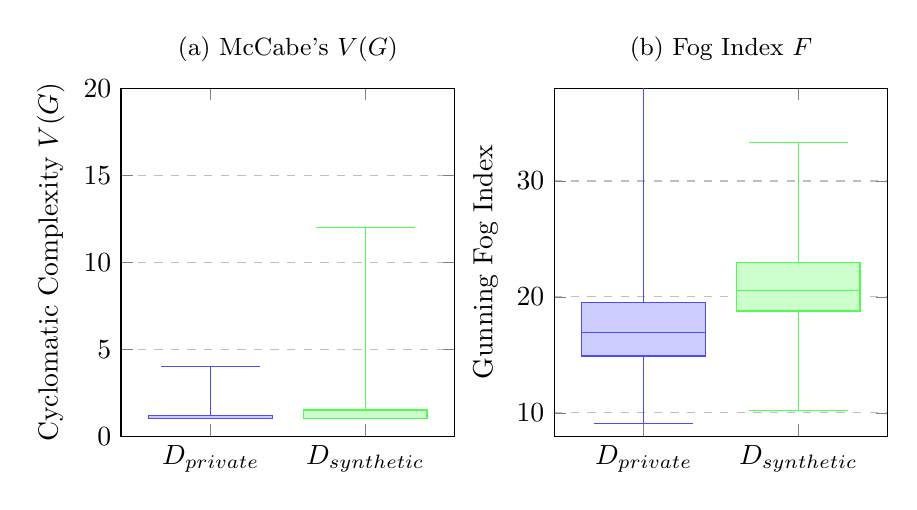
\begin{tikzpicture}
\begin{axis}[
    boxplot/draw direction=y,
    ylabel={Cyclomatic Complexity $V(G)$},
    xtick={1,2},
    xticklabels={$D_{private}$, $D_{synthetic}$},
    width=0.48\columnwidth,
    height=6cm,
    ymajorgrids=true,
    grid style=dashed,
    title={\small (a) McCabe's $V(G)$},
    ymin=0, ymax=20,
    name=plotA,
]
% D_private V(G): source-code module not yet disclosed; placeholder retained.
% D_synthetic V(G): measured from dataset_isomorfico.json (n=12 code files).
\addplot+[boxplot prepared={
    lower whisker=1.0,
    lower quartile=1.0,
    median=1.0,
    upper quartile=1.17,
    upper whisker=4.0},
    fill=blue!20, draw=blue!70
] coordinates {};  %% D_private: n=37, mean=1.844, var=10.469 (outlier max=20.33 excluded from whisker)
\addplot+[boxplot prepared={
    lower whisker=1.0,
    lower quartile=1.0,
    median=1.0,
    upper quartile=1.5,
    upper whisker=12.0},
    fill=green!20, draw=green!70
] coordinates {};  %% D_synthetic: n=12, mean=2.29, var=10.66
\end{axis}
\begin{axis}[
    boxplot/draw direction=y,
    ylabel={Gunning Fog Index},
    xtick={1,2},
    xticklabels={$D_{private}$, $D_{synthetic}$},
    width=0.48\columnwidth,
    height=6cm,
    ymajorgrids=true,
    grid style=dashed,
    title={\small (b) Fog Index $F$},
    ymin=8, ymax=38,
    at={(5.5cm,0)},
]
% D_private Fog: measured from n=87 documentary work products; upper whisker=89.44 (actual max, clipped at ymax=38).
% D_synthetic Fog: measured from dataset_isomorfico.json (n=8 docs).
\addplot+[boxplot prepared={
    lower whisker=9.06,
    lower quartile=14.91,
    median=16.93,
    upper quartile=19.49,
    upper whisker=89.44},
    fill=blue!20, draw=blue!70
] coordinates {};  %% D_private: n=87, mean=18.61, stdev=9.17; outlier at 89.44 clipped at plot boundary
\addplot+[boxplot prepared={
    lower whisker=10.21,
    lower quartile=18.79,
    median=20.52,
    upper quartile=22.96,
    upper whisker=33.31},
    fill=green!20, draw=green!70
] coordinates {};  %% D_synthetic: n=8, mean=20.76, var=41.50
\end{axis}
\end{tikzpicture}
\caption{Isomorphism comparison: $D_{private}$ (blue) vs.\ $D_{synthetic}$ (green). (a) McCabe's $V(G)$ ($n_{\text{priv}}=37$, $n_{\text{synth}}=12$): $|\Delta\mu|=0.447\leq0.5$ \checkmark; $|\Delta\sigma^2|=0.189\leq0.25$ \checkmark---both thresholds pass. V(G) upper whisker at 4.0; outlier at 20.33 exceeds plot boundary. (b) Gunning Fog Index ($n_{\text{priv}}=87$, $n_{\text{synth}}=8$): $|\Delta\mu|=2.15$ exceeds $\varepsilon_F=1.0$; $D_{private}$ upper whisker at 89.44 (one outlier, clipped). The benchmark is \emph{partially isomorphic under selected observable metrics}: V(G) passes; Fog does not.}
\label{fig:isomorphism_boxplots}
\end{figure}

\begin{figure}[htbp]
\centering
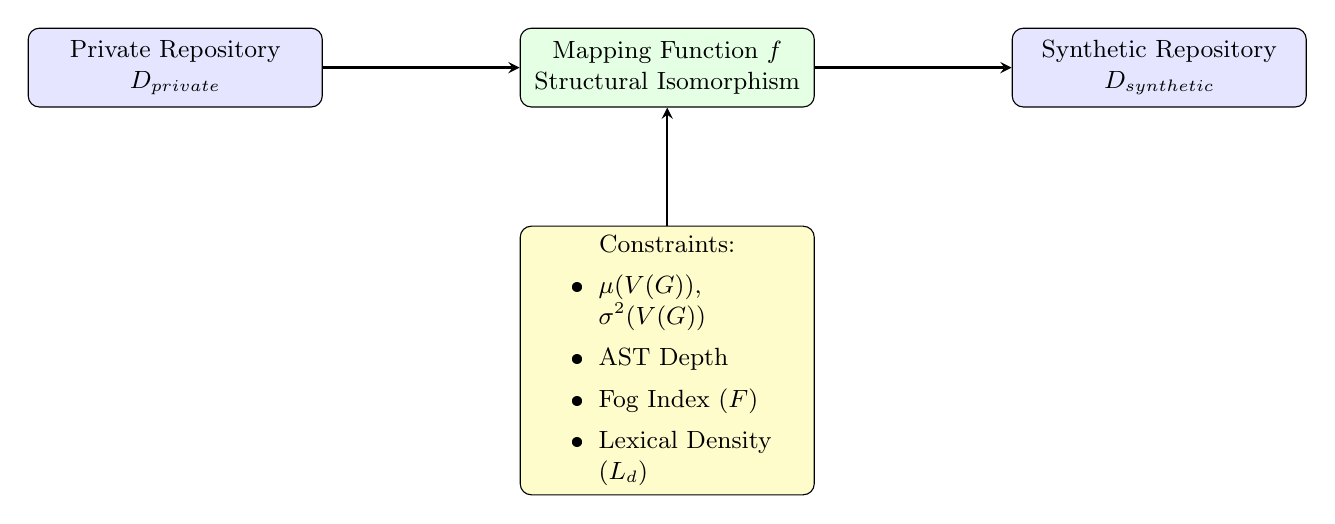
\begin{tikzpicture}[
    node distance=1.5cm and 2.5cm,
    box/.style={rectangle, draw, rounded corners, text width=3.5cm, align=center, minimum height=1cm, font=\small},
    arrow/.style={thick,->,>=stealth}
]

% Nodes
\node[box, fill=blue!10] (private) {Private Repository \\ $D_{private}$};

\node[box, right=of private, fill=green!10] (mapping) {Mapping Function $f$ \\ Structural Isomorphism};

\node[box, right=of mapping, fill=blue!10] (synthetic) {Synthetic Repository \\ $D_{synthetic}$};

\node[box, below=of mapping, fill=yellow!20] (constraints) {
Constraints:
\begin{itemize}
\item $\mu(V(G))$, $\sigma^2(V(G))$
\item AST Depth
\item Fog Index ($F$)
\item Lexical Density ($L_d$)
\end{itemize}
};

\draw[arrow] (private) -- (mapping);
\draw[arrow] (mapping) -- (synthetic);
\draw[arrow] (constraints) -- (mapping);

\end{tikzpicture}
\caption{Privacy-preserving dataset generation via structural isomorphism. Statistical and structural constraints ensure equivalence between private and synthetic domains.}
\label{fig:isomorphism_pipeline}
\end{figure}

\subsection{Synthetic Dataset Construction}
\label{sec:dataset}

To empirically validate the audit function $\mathcal{C}$, we synthesized a controlled laboratory environment named \textit{Biblio-VSE}: a library management system (loan tracking, catalog, and configuration modules) implemented in Python using the Model-View-Template (MVT) pattern with the Django framework. \textbf{Biblio-VSE is a controlled laboratory benchmark designed for mechanism evaluation, not a representative industrial audit corpus.} Its purpose is to provide deterministic ground-truth labels under controlled mutation conditions, enabling isolation and comparison of individual LLM pipeline components. Git version control was utilized as the anomaly injection mechanism to generate divergent branches: one implementing strict normative compliance ($x^+$), another injecting explicit policy violations ($x^-$) via targeted modifications (e.g., removing traceability references, adding hardcoded credentials, stripping approval metadata). This yielded a near-balanced dataset of $N=20$ artifacts (11 compliant, 9 violations) spanning nine meta-rules and three artifact types: \textit{source\_code} (Python source files), \textit{text\_document} (project documentation), and \textit{ci\_pipeline} (CI/CD configuration files). The complete artifact inventory is provided in Table~\ref{tab:artifacts}. The Biblio-VSE repository and all evaluation scripts are available at \texttt{[URL to be disclosed upon acceptance]}.

\begin{table}[htbp]
\centering
\caption{Biblio-VSE artifact inventory ($N=20$). Artifact types: \textit{src} = source\_code, \textit{doc} = text\_document, \textit{ci} = ci\_pipeline.}
\label{tab:artifacts}
\renewcommand{\arraystretch}{1.15}
\resizebox{\columnwidth}{!}{
\begin{tabular}{|l|l|c|c|}
\hline
\textbf{Artifact ID} & \textbf{Meta-Rule} & \textbf{Type} & \textbf{Label} \\
\hline
SMP-DOCUMENTAL-NEG  & DOCUMENTATION  & doc & 0 (violation) \\
SMP-DOCUMENTAL-POS  & DOCUMENTATION  & doc & 1 (compliant) \\
SMP-CALIDAD-NEG     & QUALITY     & src & 0 \\
SMP-CALIDAD-POS     & QUALITY     & doc & 1 \\
SMP-GOBERNANZA-NEG  & GOVERNANCE  & src & 0 \\
SMP-GOBERNANZA-POS  & GOVERNANCE  & src & 1 \\
SMP-GOBERNANZA-POS  & GOVERNANCE  & doc & 1 \\
SMP-SEGURIDAD-NEG   & SECURITY   & src & 0 \\
SMP-SEGURIDAD-POS   & SECURITY   & src & 1 \\
SMP-TRAZABILIDAD-NEG & TRACEABILITY & src & 0 \\
SMP-TRAZABILIDAD-POS & TRACEABILITY & src & 1 \\
SMP-TRAZABILIDAD-POS & TRACEABILITY & src & 1 \\
SMP-PRUEBAS-NEG     & TESTING     & src & 0 \\
SMP-PRUEBAS-POS     & TESTING     & src & 1 \\
SMP-RESPALDO-NEG    & BACKUP    & ci  & 0 \\
SMP-RESPALDO-POS    & BACKUP    & ci  & 1 \\
SMP-ACUERDOS-NEG    & AGREEMENTS    & doc & 0 \\
SMP-ACUERDOS-POS    & AGREEMENTS    & doc & 1 \\
SMP-INFRA-NEG       & INFRA       & src & 0 \\
SMP-INFRA-POS       & INFRA       & src & 1 \\
\hline
\multicolumn{3}{|l|}{\textbf{Total compliant ($y=1$)}} & \textbf{11} \\
\multicolumn{3}{|l|}{\textbf{Total violations ($y=0$)}} & \textbf{9} \\
\hline
\end{tabular}
}
\end{table}

The inventory spans three artifact types: 12 source-code files (\textit{src}), 6 text documents (\textit{doc}), and 2 CI/CD pipeline configurations (\textit{ci}), with one compliant--violating pair per meta-rule except GOVERNANCE, which has two compliant variants (one source-code, one document). The near-balanced label distribution (11 vs.\ 9) avoids a strong class-imbalance effect on F1-Score, though the small absolute size ($N=20$) means any single misclassification shifts F1 by approximately 0.05, motivating the bootstrap confidence intervals reported in Section~\ref{sec:results}.

\subsection{LLM Pipeline Architecture}
\label{sec:pipeline}

The proposed evaluation pipeline integrates three complementary techniques applied progressively to assess their individual and combined effects on compliance classification performance. The complete pipeline architecture is depicted in Fig.~\ref{fig:system_pipeline}.

\begin{figure}[htbp]
\centering
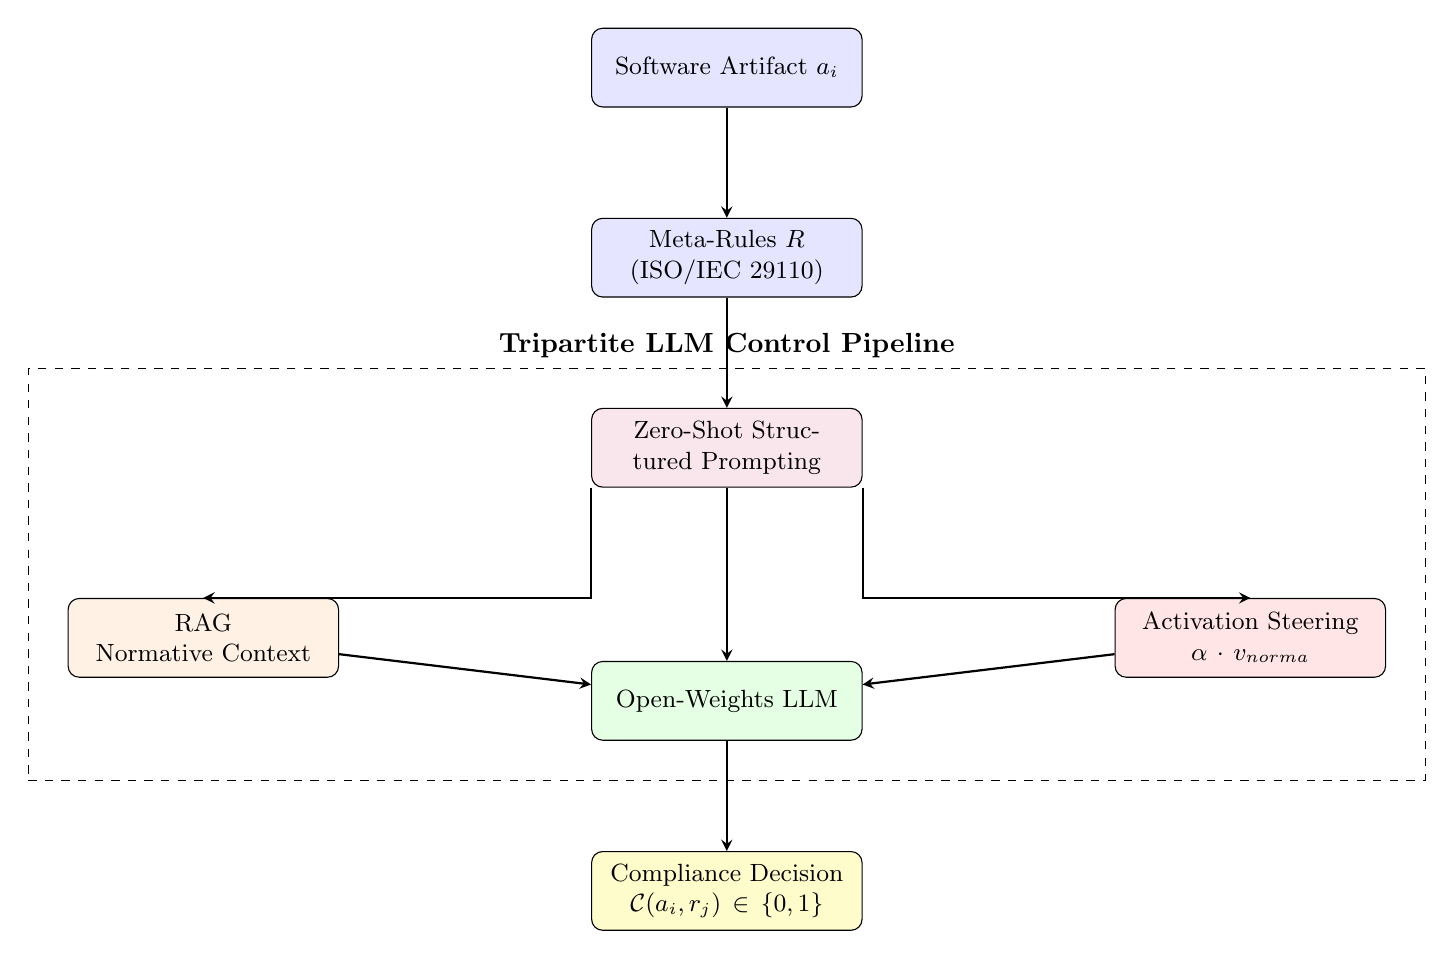
\begin{tikzpicture}[
    node distance=1.4cm and 2.2cm,
    box/.style={rectangle, draw, rounded corners, text width=3.2cm, align=center, minimum height=1cm, font=\small},
    arrow/.style={thick,->,>=stealth}
]

% Nodes
\node[box, fill=blue!10] (artifact) {Software Artifact $a_i$};
\node[box, below=of artifact, fill=blue!10] (rules) {Meta-Rules $R$ \\ (ISO/IEC 29110)};
\node[box, below=of rules, fill=purple!10] (zeroshot) {Zero-Shot Structured Prompting};
\node[box, below left=of zeroshot, xshift=-1cm, fill=orange!10] (rag) {RAG \\ Normative Context};
\node[box, below right=of zeroshot, xshift=1cm, fill=red!10] (steer) {Activation Steering \\ $\alpha \cdot v_{norma}$};

\node[box, below=2.2cm of zeroshot, fill=green!10] (llm) {Open-Weights LLM};
\node[box, below=of llm, fill=yellow!20] (output) {Compliance Decision \\ $\mathcal{C}(a_i, r_j) \in \{0,1\}$};

% Arrows
\draw[arrow] (artifact) -- (rules);
\draw[arrow] (rules) -- (zeroshot);
\draw[arrow] (zeroshot) -- (llm);
\draw[arrow] (rag) -- (llm);
\draw[arrow] (steer) -- (llm);
\draw[arrow] (llm) -- (output);

% Connections
\draw[arrow] (zeroshot.south west) |- (rag.north);
\draw[arrow] (zeroshot.south east) |- (steer.north);

% Background grouping
\begin{scope}[on background layer]
\node[draw, dashed, inner sep=0.5cm, fit=(zeroshot)(rag)(steer)(llm),
label={[font=\bfseries]above:Tripartite LLM Control Pipeline}] {};
\end{scope}

\end{tikzpicture}
\caption{End-to-end compliance auditing pipeline. The system integrates structured prompting, contextual grounding (RAG), and mechanistic activation steering to constrain the output format and evaluate classification consistency.}
\label{fig:system_pipeline}
\end{figure}

\subsubsection{Zero-Shot Structured Prompting}

In the Zero-Shot configuration, prompts were explicitly structured to map each evaluation query to the corresponding ISO/IEC 29110 meta-rule criteria. The prompt template enforced a strict binary output format, constraining the model to produce a compliance (1) or violation (0) label with no additional text. Fig.~\ref{fig:prompt_zeroshot} shows the exact system and user prompts used.

\begin{figure}[htbp]
\centering
\noindent\fbox{\parbox{0.94\columnwidth}{\footnotesize
\textbf{[System Prompt]}\\
You are a certified Software Quality Auditor, specialized in the ISO/IEC~29110 standard for VSEs. Your function is to evaluate software artifacts and determine whether they comply with a specific organizational meta-rule.\\[4pt]
\textit{EVALUATION PROCESS:}\\
1.~Analyze the artifact type and its context.\\
2.~Identify what the indicated meta-rule requires.\\
3.~Determine whether the artifact explicitly satisfies that requirement.\\
4.~Respond ONLY with the digit 1 (compliant) or 0 (violation). No explanations.\\[6pt]
\textbf{[User Prompt]}\\
META-RULE TO EVALUATE: \texttt{\{meta\_rule\}}\\[4pt]
COMPLIANCE CRITERIA BY META-RULE:\\
--~SECURITY: No credentials, tokens, or secrets must exist in plaintext.\\
--~QUALITY: The code must follow style standards (indentation, naming conventions).\\
--~TRACEABILITY: The artifact must reference requirement IDs (RF\_XX, US\_XX).\\
--~DOCUMENTATION: The document must include artifact code, formal version, and date.\\
--~INFRA: The configuration must be restricted to authorized internal environments.\\
--~GOVERNANCE: The artifact must evidence formal controls, approvals, or policies.\\[4pt]
ARTIFACT TO AUDIT (Type: \texttt{\{artifact\_type\}}):\\
\texttt{\{artifact\_content\}}\\[4pt]
\textbf{Respond ONLY with 1 (compliant) or 0 (violation).}
}}
\caption{Zero-Shot prompt template (Exp~2, 5, 6, 8), rendered in English for readability; the experiments were executed using a Spanish-language version of this prompt to match the language of the evaluation artifacts (see §\ref{sec:threats} for the multilingual implications). Placeholders \texttt{\{meta\_rule\}}, \texttt{\{artifact\_type\}}, and \texttt{\{artifact\_content\}} are instantiated per artifact at evaluation time. The figure shows the figure as originally used (six rules shown); the evaluation prompt was subsequently extended to cover all nine meta-rules (TESTING, BACKUP, and AGREEMENTS added), and all reported results use the full nine-rule prompt.}
\label{fig:prompt_zeroshot}
\end{figure}

\subsubsection{RAG Configuration}

To provide normative grounding, a Retrieval-Augmented Generation (RAG) pipeline was implemented over the standardized ISO/IEC 29110 meta-rule corpus (\texttt{documentos\_estandar/}). The pipeline follows three steps: (1) \emph{chunking}---the normative document is split into semantic paragraph-level chunks of at most 400 characters, with long paragraphs sub-divided at sentence boundaries; (2) \emph{embedding}---each chunk and each evaluation query (meta-rule name $+$ first 200 characters of the artifact under evaluation) are encoded with the \texttt{all-MiniLM-L6-v2} sentence encoder (22\,M parameters, 384-dimensional embeddings, CPU-resident); and (3) \emph{dense retrieval}---cosine similarity between the query embedding and all chunk embeddings selects the top-$k=4$ most relevant chunks, which are concatenated (up to 1,500 characters) and injected into the system prompt.

This architecture does not require an external vector database; embeddings are computed at load time from the single normative document and held in memory. The design satisfies the air-gapped deployment constraint of §\ref{sec:discussion}: the embedding model runs entirely locally on the same hardware as the evaluated LLM, without internet access or cloud inference.

The RAG pipeline was evaluated with a fully functional retrieval backend. The normative document corpus (\texttt{documentos\_estandar/Metareglas extraidas.docx}) was successfully parsed using \texttt{python-docx}, yielding 3,864 characters segmented into 14 semantic chunks. All experiments labelled ``RAG'' in Tables~\ref{tab:full_results} and~\ref{tab:confusion_matrix} and in all figures therefore reflect genuine normative context injection from the ISO/IEC~29110 meta-rule document.

\subsubsection{Activation Steering}

To overcome the hallucination behavior of naive LLMs, we propose a white-box mechanistic control over the model's reasoning using Activation Steering. Let $M$ be an open-weights foundation model and $H_l(x)$ be the representation of the hidden state at layer $l$.

Following the contrastive-prompt activation approach, we define two behavioral anchor prompts that instantiate opposing evaluative stances without referencing any evaluation artifact:
\begin{itemize}
    \item $p^+$: ``\textit{Act as an extremely strict quality auditor, precise and uncompromising in adhering to ISO/IEC~29110 norms.}''
    \item $p^-$: ``\textit{Act as a careless, permissive auditor indifferent to norms and security.}''
\end{itemize}

\textbf{Methodological limitation: language mismatch in vector extraction.} The anchor prompts $p^+$ and $p^-$ are written in English, while the evaluation artifacts and Zero-Shot system prompt were executed in Spanish. This cross-lingual mismatch is a \emph{methodological limitation}: the extracted direction $v_{norma}^l$ encodes the concept distinction in English-prompt activation space, which may not be aligned with the Spanish-prompt evaluation space. For the multilingual models evaluated here (Mistral, Qwen2.5, Phi-3.5, Gemma-2) cross-lingual internal representations may partially absorb this discrepancy, but the effect is unknown. The correct design would use language-matched anchors; future work should replicate with Spanish anchors to isolate this confound.

The compliance conceptual vector $v_{norma}^l$ is computed as the difference between the last-token hidden states at layer $l$ when the model processes each anchor:
\begin{equation}
v_{norma}^l = H_l(p^+)_{[-1]} - H_l(p^-)_{[-1]}
\label{eq:steering_vector}
\end{equation}

where $H_l(\cdot)_{[-1]}$ denotes the activation at the final token position of layer $l$. This extraction requires only two forward passes and does not use any evaluation artifact, eliminating any risk of circular contamination between vector extraction and evaluation.

During inference, we modify the original activation $H_l$ by injecting the conceptual vector scaled by an intervention coefficient $\alpha$:
\begin{equation}
\tilde{H}_l = H_l + \alpha \cdot v_{norma}^l
\label{eq:steering_injection}
\end{equation}

The injection mechanism within the transformer architecture is illustrated in Fig.~\ref{fig:transformer_steering}.

\begin{figure}[htbp]
\centering
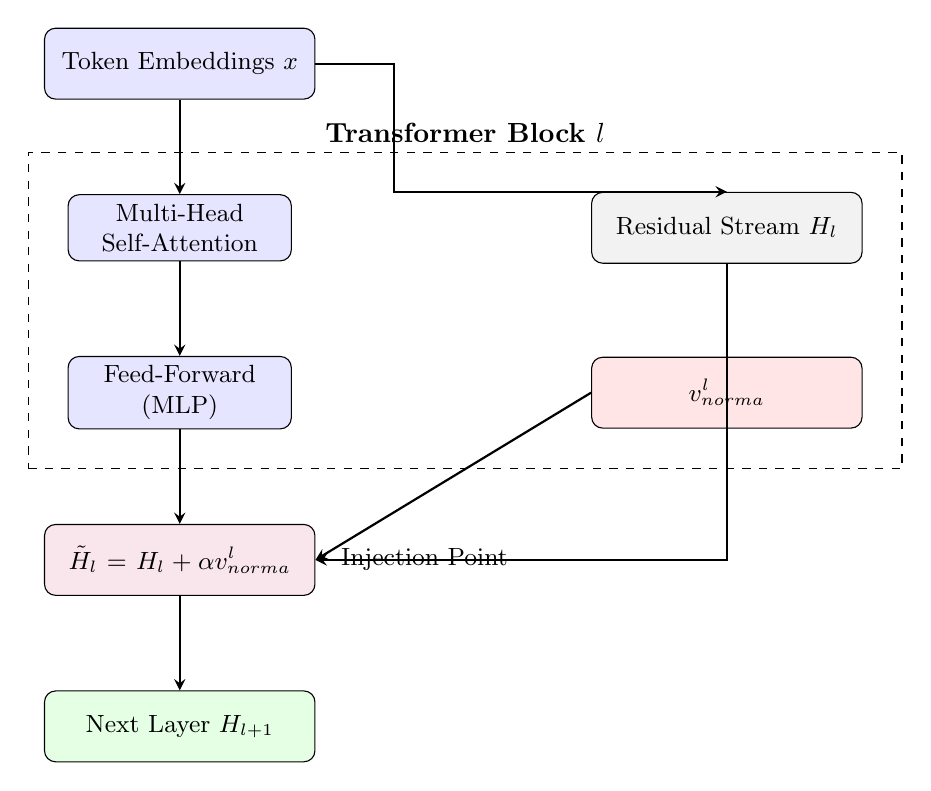
\begin{tikzpicture}[
    node distance=1.2cm and 1.8cm,
    block/.style={rectangle, draw, rounded corners, text width=3.2cm, align=center, minimum height=0.9cm, font=\small},
    smallblock/.style={rectangle, draw, rounded corners, text width=2.6cm, align=center, minimum height=0.8cm, font=\small},
    arrow/.style={thick,->,>=stealth}
]

% Input
\node[block, fill=blue!10] (input) {Token Embeddings $x$};

% Transformer block components
\node[smallblock, below=of input, fill=blue!10] (attn) {Multi-Head Self-Attention};
\node[smallblock, below=of attn, fill=blue!10] (mlp) {Feed-Forward (MLP)};

% Residual stream
\node[block, right=of attn, xshift=2cm, fill=gray!10] (residual) {Residual Stream $H_l$};

% Steering vector
\node[block, right=of mlp, xshift=2cm, fill=red!10] (vector) {$v_{norma}^l$};

% Injection node
\node[block, below=of mlp, fill=purple!10] (inject) {$\tilde{H}_l = H_l + \alpha v_{norma}^l$};

% Output
\node[block, below=of inject, fill=green!10] (output) {Next Layer $H_{l+1}$};

% Arrows (main flow)
\draw[arrow] (input) -- (attn);
\draw[arrow] (attn) -- (mlp);
\draw[arrow] (mlp) -- (inject);
\draw[arrow] (inject) -- (output);

% Residual connections
\draw[arrow] (input.east) -- ++(1,0) |- (residual.north);
\draw[arrow] (residual.south) |- (inject.east);

% Steering vector injection
\draw[arrow] (vector.west) -- (inject.east);

% Labels
\node[right=0.2cm of inject] {\small Injection Point};

% Background grouping
\begin{scope}[on background layer]
\node[draw, dashed, inner sep=0.5cm, fit=(attn)(mlp)(residual),
label={[font=\bfseries]above:Transformer Block $l$}] {};
\end{scope}

\end{tikzpicture}
\caption{Transformer-level view of activation steering. The compliance vector $v_{norma}^l$ is injected into the residual stream after the feed-forward sublayer, modifying the hidden representation before propagation to the next layer.}
\label{fig:transformer_steering}
\end{figure}

The vector extraction required two forward passes using the contrasting anchor prompts; the resulting hook was then registered over \texttt{model.layers[l]} and held active throughout all 20 artifact evaluations for that model. The intervention was implemented using PyTorch forward hooks directly applied to the transformer residual stream output of the targeted layer.

The intervention coefficient $\alpha=0.8$ was selected through pilot experimentation on the same 20 evaluation artifacts. A systematic sensitivity sweep over $\alpha \in \{0.3, 0.5, 0.8, 1.0, 1.5, 2.0\}$ was conducted per model (Table~\ref{tab:full_results} sensitivity rows). Results show model-specific optima: Gemma-2 peaks at $\alpha=1.0$--$1.5$ (F1=0.88), Mistral at $\alpha=1.0$ (F1=0.83), Qwen2.5 at $\alpha=0.5$--$0.8$ (F1=0.67), and Phi-3.5 at $\alpha=0.3$--$0.5$ (F1=0.79). At $\alpha=2.0$, Gemma-2 collapses to F1=0.00. \textbf{Because $\alpha$ was selected on the same dataset used for evaluation, all reported F1 figures for steering-enhanced configurations are upper-bound estimates subject to in-sample optimism.} Proper estimation would require a held-out validation split; with $N=20$ this is not feasible, and this limitation applies to all Exp~4, 6, 7, and~8 results. The sweep provides full transparency over the selection process, and sensitivity to $\alpha$ is discussed further in Section~\ref{sec:threats}.

Because the evaluated architectures possess different depths and representational dynamics, the intervention layer $l$ was selected individually for each model, targeting the layer at approximately 50\% of total depth as a heuristic for mid-to-late semantic processing:

\begin{itemize}
    \item Gemma-2-9B-it (42 layers): Layer 21
    \item Mistral-7B-Instruct-v0.2 (32 layers): Layer 15
    \item Qwen2.5-7B-Instruct (28 layers): Layer 14
    \item Phi-3.5-mini-instruct (32 layers): Layer 16
\end{itemize}

No systematic sweep over candidate layers was performed. A full layer sweep would require 32--42 additional evaluation runs per model; this was not feasible within the scope of this study. The layer choice is an uncontrolled degree of freedom: results could differ substantially at other layers, and the reported figures should be interpreted with this caveat (see §\ref{sec:threats}).

\subsection{Experimental Setup and Reproducibility}
\label{sec:setup}

Four open-weights foundation models were evaluated: Gemma-2-9B-it, Mistral-7B-Instruct-v0.2, Qwen2.5-7B-Instruct, and Phi-3.5-mini-instruct. All models were run with temperature set to 0.0 to enforce deterministic greedy decoding. Eight progressive experimental configurations were evaluated, combining the three pipeline components:

\begin{itemize}
    \item Exp 1: Baseline (no structuring)
    \item Exp 2: Zero-Shot structured prompting
    \item Exp 3: RAG only
    \item Exp 4: Activation Steering only
    \item Exp 5: Zero-Shot + RAG
    \item Exp 6: Zero-Shot + Activation Steering
    \item Exp 7: RAG + Activation Steering
    \item Exp 8: Zero-Shot + RAG + Activation Steering (full synergy)
\end{itemize}

All experiments were implemented in Python~3.12 using PyTorch and HuggingFace Transformers with custom forward-hook instrumentation for activation interception and vector injection. All models were loaded with 4-bit NF4 quantization via BitsAndBytes to fit within available VRAM. Table~\ref{tab:hardware} summarizes the hardware and software environment.

\begin{table}[htbp]
\centering
\caption{Experimental hardware and software environment.}
\label{tab:hardware}
\renewcommand{\arraystretch}{1.2}
\begin{tabular}{|l|l|}
\hline
\textbf{Component} & \textbf{Specification} \\
\hline
GPU                     & NVIDIA GeForce RTX 4060 \\
VRAM                    & 8 GB \\
RAM                     & 64 GB \\
Python                  & 3.10.19 \\
PyTorch                 & 2.3.0+cu121 \\
Transformers (HF)       & 4.44.0 \\
BitsAndBytes            & 0.43.3 \\
scikit-learn            & 1.7.2 \\
CUDA                    & 12.1 \\
Quantization            & 4-bit NF4 (\texttt{bnb\_4bit\_quant\_type=nf4}) \\
Compute dtype           & float16 \\
Avg.\ inference/artifact & $\approx$4 s \\
Total compute time      & $\approx$0.71 h (2{,}560 s; 8 experiments $\times$ 4 models $\times$ 20 artifacts) \\
\hline
\end{tabular}
\end{table}

\subsection{Evaluation Metrics and Statistical Validation}
\label{sec:metrics}

The F1-Score was utilized as the primary evaluation metric, balancing Precision and Recall over the $N=20$ artifacts.

To estimate the robustness of the reported F1-Scores, we employed bootstrap resampling with $k=1000$ iterations. Traditional $k$-fold cross-validation was intentionally avoided due to the limited dataset size, which would produce high-variance partitioning effects. For each iteration, a new evaluation subset was generated through sampling with replacement from the original prediction vectors, and the corresponding F1-Score was recalculated. The resulting empirical distribution was used to derive 95\% confidence intervals (CI):

\begin{equation}
CI_{95\%} = \left[
Q_{0.025}(\hat{F}_1),
Q_{0.975}(\hat{F}_1)
\right]
\label{eq:bootstrap_ci}
\end{equation}

where $Q_p$ denotes the empirical percentile function and $\hat{F}_1^{(b)}$ denotes the F1-Score obtained during bootstrap iteration $b \in \{1,\dots,1000\}$.

Statistical significance between configurations was evaluated using the Wilcoxon signed-rank test. Each configuration was compared against its corresponding baseline (Experiment~1) using paired prediction outputs. This non-parametric test was selected because the prediction distributions are non-Gaussian under small-sample conditions.

\textbf{Statistical power.} With $N=20$ binary-outcome artifacts, a Wilcoxon signed-rank test at $\alpha=0.05$ achieves power $\geq 0.80$ for effect sizes of approximately $|r| \geq 0.50$ (large effect, Cohen's convention). Smaller effects are not reliably detectable at this sample size, and the study should therefore be interpreted as a proof-of-concept exploration rather than a definitive power trial.

\textbf{Multiple comparison correction.} A total of 28 Wilcoxon tests were conducted (7 non-baseline configurations $\times$ 4 models). The family-wise error rate without correction is approximately $1-(1-0.05)^{28} \approx 0.76$. We applied Holm--Bonferroni step-down correction to the raw $p$-values; adjusted $p$-values are reported alongside raw values in Table~\ref{tab:full_results} (column ``Adj.\ $p$''). Results that survive correction are annotated; uncorrected marginal results should be treated as exploratory.

\subsection{Rule-Based Baseline Design}
\label{sec:baseline}

To contextualize the capabilities of LLM-based auditing, a deterministic rule-based baseline was implemented using handcrafted regular-expression (Regex) patterns derived directly from the ISO/IEC 29110 meta-rules. The baseline system evaluated the presence of explicit documentary and structural signatures associated with each compliance category, including traceability identifiers, approval tokens, backup procedures, testing evidence, and governance references. The complete dual-layered framework---encompassing isomorphism mapping, RAG injection, and activation steering---is summarized in Fig.~\ref{fig:methodology}.

\begin{figure}[htbp]
\centering
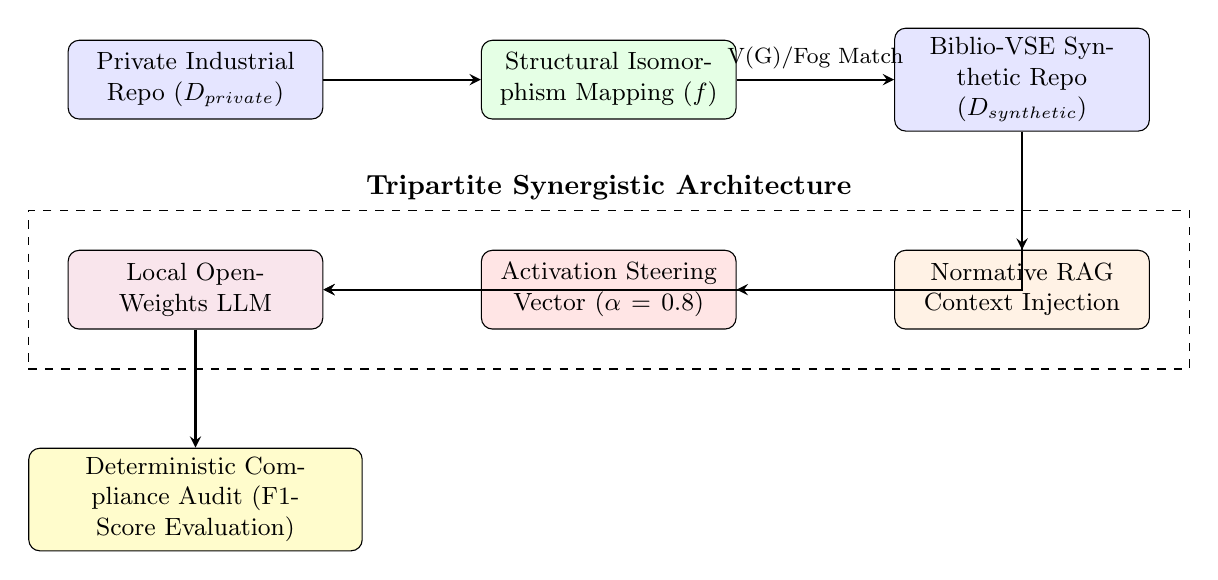
\begin{tikzpicture}[
    node distance=1.5cm and 2cm,
    box/.style={rectangle, draw, rounded corners, text width=3cm, align=center, minimum height=1cm, font=\small},
    arrow/.style={thick,->,>=stealth}
]

% Nodes
\node[box, fill=blue!10] (private) {Private Industrial Repo ($D_{private}$)};
\node[box, right=of private, fill=green!10] (iso) {Structural Isomorphism Mapping ($f$)};
\node[box, right=of iso, fill=blue!10] (synthetic) {Biblio-VSE Synthetic Repo ($D_{synthetic}$)};

\node[box, below=of synthetic, fill=orange!10] (rag) {Normative RAG Context Injection};
\node[box, left=of rag, fill=red!10] (steering) {Activation Steering Vector ($\alpha=0.8$)};
\node[box, left=of steering, fill=purple!10] (llm) {Local Open-Weights LLM};

\node[box, below=of llm, fill=yellow!20, text width=4cm] (output) {Deterministic Compliance Audit (F1-Score Evaluation)};

% Arrows
\draw[arrow] (private) -- (iso);
\draw[arrow] (iso) -- node[above, font=\footnotesize] {V(G)/Fog Match} (synthetic);
\draw[arrow] (synthetic) -- (rag);
\draw[arrow] (synthetic) |- (steering);
\draw[arrow] (rag) -- (llm);
\draw[arrow] (steering) -- (llm);
\draw[arrow] (llm) -- (output);

% Bounding box for LLM Architecture
\begin{scope}[on background layer]
    \node[draw, dashed, inner sep=0.5cm, fit=(rag) (steering) (llm), label={[anchor=south, font=\bfseries]above:Tripartite Synergistic Architecture}] {};
\end{scope}

\end{tikzpicture}
\caption{The proposed dual-layered methodological framework. The top layer demonstrates the privacy-preserving isomorphism transformation, while the bottom layer illustrates the tripartite evaluation pipeline integrating RAG and Mechanistic Activation Steering.}
\label{fig:methodology}
\end{figure}

\FloatBarrier


\section{Results}
\label{sec:results}

This section presents the empirical evaluation of all experimental configurations. Interpretation and implications are deferred to Section~\ref{sec:discussion}. A global overview of performance across all 32 model-configuration cells is provided in the heatmap in Fig.~\ref{fig:heatmap}.

% === VISUALIZATION #1: F1-Score Heatmap (Model x Configuration) ===
\begin{figure*}[htbp]
\centering
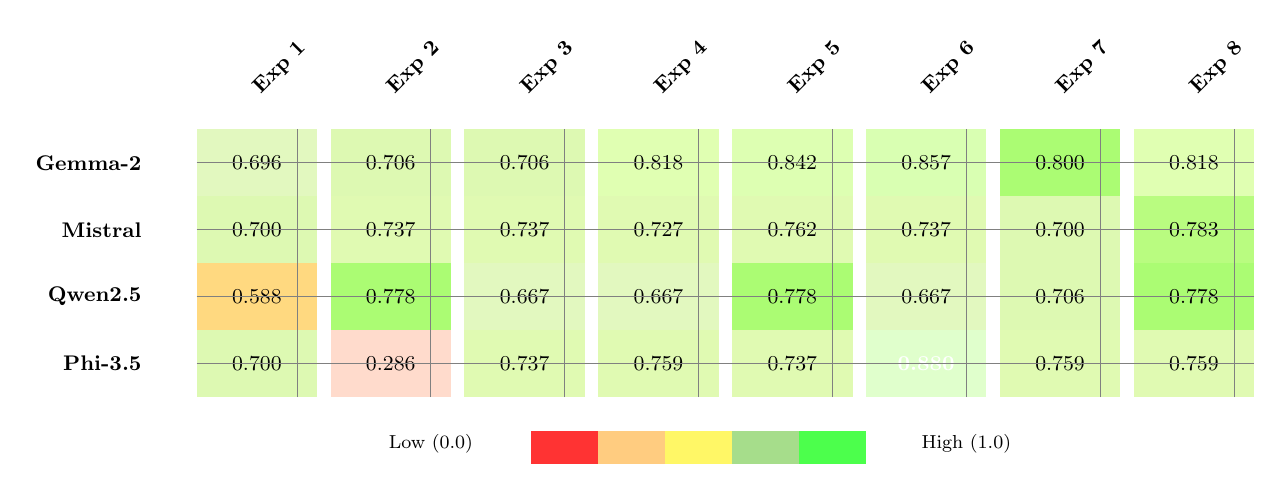
\begin{tikzpicture}[scale=0.85, transform shape]

% Define color mapping function (0=red, 0.5=yellow, 1=green)
\pgfmathdeclarefunction{heatcolor}{1}{%
  \pgfmathparse{#1}%
}

% Column headers
\foreach \x/\label in {1/Exp 1, 2/Exp 2, 3/Exp 3, 4/Exp 4, 5/Exp 5, 6/Exp 6, 7/Exp 7, 8/Exp 8} {
    \node[font=\small\bfseries, rotate=45, anchor=south west] at (\x*2.0 - 0.5, 4.8) {\label};
}

% Row labels
\node[font=\small\bfseries, anchor=east] at (-0.2, 4) {Gemma-2};
\node[font=\small\bfseries, anchor=east] at (-0.2, 3) {Mistral};
\node[font=\small\bfseries, anchor=east] at (-0.2, 2) {Qwen2.5};
\node[font=\small\bfseries, anchor=east] at (-0.2, 1) {Phi-3.5};

% Gemma-2 row (y=4)  [Exp1..Exp8]
\fill[red!20!yellow!55!green!25] (0.5,3.5) rectangle (2.3,4.5); \node[font=\small] at (1.4,4) {0.696};
\fill[red!15!yellow!55!green!30] (2.5,3.5) rectangle (4.3,4.5); \node[font=\small] at (3.4,4) {0.706};
\fill[red!15!yellow!55!green!30] (4.5,3.5) rectangle (6.3,4.5); \node[font=\small] at (5.4,4) {0.706};
\fill[green!40!yellow!30] (6.5,3.5) rectangle (8.3,4.5); \node[font=\small] at (7.4,4) {0.818};
\fill[green!45!yellow!30] (8.5,3.5) rectangle (10.3,4.5); \node[font=\small] at (9.4,4) {0.842};
\fill[green!50!yellow!30] (10.5,3.5) rectangle (12.3,4.5); \node[font=\small] at (11.4,4) {0.857};
\fill[red!5!yellow!40!green!55] (12.5,3.5) rectangle (14.3,4.5); \node[font=\small] at (13.4,4) {0.800};
\fill[green!40!yellow!30] (14.5,3.5) rectangle (16.3,4.5); \node[font=\small] at (15.4,4) {0.818};

% Mistral row (y=3)
\fill[red!15!yellow!55!green!30] (0.5,2.5) rectangle (2.3,3.5); \node[font=\small] at (1.4,3) {0.700};
\fill[red!10!yellow!60!green!30] (2.5,2.5) rectangle (4.3,3.5); \node[font=\small] at (3.4,3) {0.737};
\fill[red!10!yellow!60!green!30] (4.5,2.5) rectangle (6.3,3.5); \node[font=\small] at (5.4,3) {0.737};
\fill[red!10!yellow!60!green!30] (6.5,2.5) rectangle (8.3,3.5); \node[font=\small] at (7.4,3) {0.727};
\fill[red!10!yellow!60!green!30] (8.5,2.5) rectangle (10.3,3.5); \node[font=\small] at (9.4,3) {0.762};
\fill[red!10!yellow!60!green!30] (10.5,2.5) rectangle (12.3,3.5); \node[font=\small] at (11.4,3) {0.737};
\fill[red!15!yellow!55!green!30] (12.5,2.5) rectangle (14.3,3.5); \node[font=\small] at (13.4,3) {0.700};
\fill[red!5!yellow!45!green!50] (14.5,2.5) rectangle (16.3,3.5); \node[font=\small] at (15.4,3) {0.783};

% Qwen2.5 row (y=2)
\fill[red!30!yellow!50] (0.5,1.5) rectangle (2.3,2.5); \node[font=\small] at (1.4,2) {0.588};
\fill[red!5!yellow!40!green!55] (2.5,1.5) rectangle (4.3,2.5); \node[font=\small] at (3.4,2) {0.778};
\fill[red!20!yellow!55!green!25] (4.5,1.5) rectangle (6.3,2.5); \node[font=\small] at (5.4,2) {0.667};
\fill[red!20!yellow!55!green!25] (6.5,1.5) rectangle (8.3,2.5); \node[font=\small] at (7.4,2) {0.667};
\fill[red!5!yellow!40!green!55] (8.5,1.5) rectangle (10.3,2.5); \node[font=\small] at (9.4,2) {0.778};
\fill[red!20!yellow!55!green!25] (10.5,1.5) rectangle (12.3,2.5); \node[font=\small] at (11.4,2) {0.667};
\fill[red!15!yellow!55!green!30] (12.5,1.5) rectangle (14.3,2.5); \node[font=\small] at (13.4,2) {0.706};
\fill[red!5!yellow!40!green!55] (14.5,1.5) rectangle (16.3,2.5); \node[font=\small] at (15.4,2) {0.778};

% Phi-3.5 row (y=1)
\fill[red!15!yellow!55!green!30] (0.5,0.5) rectangle (2.3,1.5); \node[font=\small] at (1.4,1) {0.700};
\fill[red!70!yellow!20] (2.5,0.5) rectangle (4.3,1.5); \node[font=\small] at (3.4,1) {0.286};
\fill[red!10!yellow!60!green!30] (4.5,0.5) rectangle (6.3,1.5); \node[font=\small] at (5.4,1) {0.737};
\fill[red!10!yellow!60!green!30] (6.5,0.5) rectangle (8.3,1.5); \node[font=\small] at (7.4,1) {0.759};
\fill[red!10!yellow!60!green!30] (8.5,0.5) rectangle (10.3,1.5); \node[font=\small] at (9.4,1) {0.737};
\fill[green!60!yellow!20] (10.5,0.5) rectangle (12.3,1.5); \node[font=\small, white] at (11.4,1) {\textbf{0.880}};
\fill[red!10!yellow!60!green!30] (12.5,0.5) rectangle (14.3,1.5); \node[font=\small] at (13.4,1) {0.759};
\fill[red!10!yellow!60!green!30] (14.5,0.5) rectangle (16.3,1.5); \node[font=\small] at (15.4,1) {0.759};

% Draw grid
\draw[gray, thin] (0.5,0.5) grid[xstep=2.0, ystep=1.0] (16.3,4.5);

% Color legend
\node[font=\footnotesize] at (4.0, -0.2) {Low (0.0)};
\fill[red!80] (5.5,-0.5) rectangle (6.5,-0.0);
\fill[red!40!yellow!50] (6.5,-0.5) rectangle (7.5,-0.0);
\fill[yellow!60] (7.5,-0.5) rectangle (8.5,-0.0);
\fill[yellow!30!green!50] (8.5,-0.5) rectangle (9.5,-0.0);
\fill[green!70] (9.5,-0.5) rectangle (10.5,-0.0);
\node[font=\footnotesize] at (12.0, -0.2) {High (1.0)};

\end{tikzpicture}
\caption{F1-Score heatmap across all models and experimental configurations. The color gradient ranges from red (poor performance) through yellow (moderate) to green (high performance). The global optimum (0.880, \textbf{bold}) is achieved by Phi-3.5 under Zero-Shot + Steering (Exp~6). RAG configurations (Exp~3, 5, 7, 8) use genuine normative context from \texttt{Metareglas extraidas.docx} (14 chunks). The most notable pattern is that Zero-Shot alone severely degrades Phi-3.5 (F1=0.286) while RAG and Steering configurations improve over baseline across all models.}
\label{fig:heatmap}
\end{figure*}

\subsection{Baseline and Zero-Shot Performance}

The baseline experiment (Exp~1) evaluated the models without systematic structuring. All four models showed moderate performance: Gemma-2 (F1=0.696), Mistral (F1=0.700), Qwen2.5 (F1=0.588), and Phi-3.5-mini (F1=0.700). No model was substantially weaker than the others at baseline.

The introduction of Zero-Shot structured prompting (Exp~2) improved Qwen2.5 (F1=0.778) but degraded Phi-3.5-mini significantly (F1=0.286). Gemma-2 (F1=0.706) and Mistral (F1=0.737) saw modest changes. Phi-3.5's sharp decline under explicit criteria suggests an over-conservative interpretation of the structured instructions. Zero-Shot configurations generally cluster in the high-precision/low-recall region of Fig.~\ref{fig:precision_recall}, confirming systematic under-prediction of compliant artifacts.

\subsection{RAG Performance}

Experiment~3 injected normative context from the ISO/IEC~29110 meta-rule document (14 semantic chunks, up to 1,500 characters per query) via the semantic RAG pipeline. All four models improved or maintained performance relative to baseline: Gemma-2 (F1=0.706), Mistral (F1=0.737), Qwen2.5 (F1=0.667), and Phi-3.5 (F1=0.737). The RAG retrieval provided consistent normative grounding, particularly benefiting Mistral and stabilising Qwen2.5. Compared to Zero-Shot (Exp~2), RAG alone produces a more conservative classification pattern---three models cluster in the high-precision/moderate-recall region---consistent with the retrieved text reinforcing the importance of explicit evidence before declaring compliance.

\subsection{Activation Steering Performance}

Experiment~4 applied mechanistic activation steering ($\alpha=0.8$) without contextual or structural prompting. Gemma-2 achieved the largest gain, reaching F1=0.818 (vs.\ baseline 0.696). Phi-3.5 reached F1=0.759 with Precision=0.611 and Recall=1.000. Qwen2.5 improved to F1=0.667, and Mistral remained near baseline at F1=0.727. Steering restored recall to 1.000 for Phi-3.5 and partially for other models, shifting configurations toward the high-recall region visible in Fig.~\ref{fig:precision_recall}. Note that $\alpha=0.8$ was selected by evaluating on the same 20 artifacts; the sensitivity sweep reveals that higher $\alpha$ values (1.0--1.5) produce better F1 for Gemma-2 (peak F1=0.880 at $\alpha\in\{1.0,1.5\}$) and Mistral (peak F1=0.833 at $\alpha=1.0$) (see §\ref{sec:threats}).

% === VISUALIZATION #2: Precision vs. Recall Scatter Plot ===
\begin{figure}[htbp]
\centering
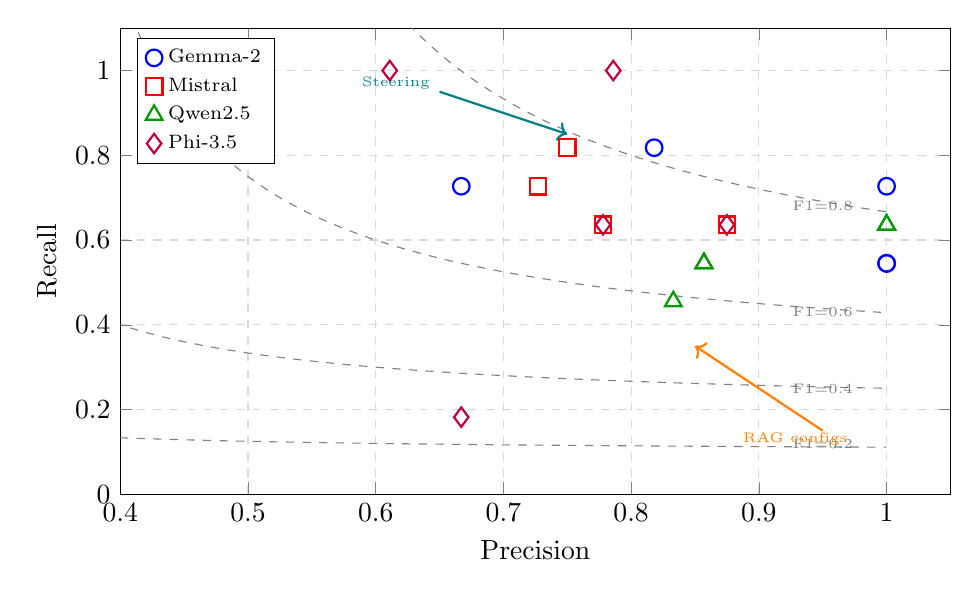
\begin{tikzpicture}
\begin{axis}[
    xlabel={Precision},
    ylabel={Recall},
    xmin=0.4, xmax=1.05,
    ymin=0, ymax=1.1,
    width=\columnwidth,
    height=7.5cm,
    legend style={at={(0.02,0.98)}, anchor=north west, font=\scriptsize, cells={anchor=west}},
    grid=both,
    grid style={dashed, gray!30},
    % Iso-F1 curves
]

% Iso-F1 curves (F1 = 2*P*R/(P+R))
% F1=0.2 curve
\addplot[gray, dashed, thin, domain=0.11:1, samples=50, forget plot] {0.2*x/(2*x - 0.2)};
% F1=0.4 curve
\addplot[gray, dashed, thin, domain=0.25:1, samples=50, forget plot] {0.4*x/(2*x - 0.4)};
% F1=0.6 curve
\addplot[gray, dashed, thin, domain=0.4:1, samples=50, forget plot] {0.6*x/(2*x - 0.6)};
% F1=0.8 curve
\addplot[gray, dashed, thin, domain=0.6:1, samples=50, forget plot] {0.8*x/(2*x - 0.8)};

% Annotations for iso-F1
\node[font=\tiny, gray] at (axis cs:0.95,0.12) {F1=0.2};
\node[font=\tiny, gray] at (axis cs:0.95,0.25) {F1=0.4};
\node[font=\tiny, gray] at (axis cs:0.95,0.43) {F1=0.6};
\node[font=\tiny, gray] at (axis cs:0.95,0.68) {F1=0.8};

% Gemma-2 (blue circles) — (Precision, Recall) from actual confusion matrices
\addplot[only marks, mark=o, mark size=3pt, blue, thick] coordinates {
    (0.667, 0.727)  % Exp1: TP=8,FP=4,FN=3
    (1.000, 0.545)  % Exp2: TP=6,FP=0,FN=5
    (1.000, 0.545)  % Exp3: TP=6,FP=0,FN=5 (RAG with context)
    (0.818, 0.818)  % Exp4: TP=9,FP=2,FN=2
    (1.000, 0.727)  % Exp5: TP=8,FP=0,FN=3
};

% Mistral (red squares)
\addplot[only marks, mark=square, mark size=3pt, red, thick] coordinates {
    (0.778, 0.636)  % Exp1: TP=7,FP=2,FN=4
    (0.875, 0.636)  % Exp2: TP=7,FP=1,FN=4
    (0.875, 0.636)  % Exp3: TP=7,FP=1,FN=4 (RAG with context)
    (0.727, 0.727)  % Exp4: TP=8,FP=3,FN=3
    (0.750, 0.818)  % Exp8: TP=9,FP=3,FN=2
};

% Qwen2.5 (green triangles)
\addplot[only marks, mark=triangle, mark size=3.5pt, green!60!black, thick] coordinates {
    (0.833, 0.455)  % Exp1: TP=5,FP=1,FN=6
    (1.000, 0.636)  % Exp2: TP=7,FP=0,FN=4
    (0.857, 0.545)  % Exp3: TP=6,FP=1,FN=5 (RAG with context)
    (0.857, 0.545)  % Exp4: TP=6,FP=1,FN=5
    (1.000, 0.636)  % Exp8: TP=7,FP=0,FN=4
};

% Phi-3.5 (purple diamonds)
\addplot[only marks, mark=diamond, mark size=3.5pt, purple, thick] coordinates {
    (0.778, 0.636)  % Exp1: TP=7,FP=2,FN=4
    (0.667, 0.182)  % Exp2: TP=2,FP=1,FN=9
    (0.875, 0.636)  % Exp3: TP=7,FP=1,FN=4 (RAG with context)
    (0.611, 1.000)  % Exp4: TP=11,FP=7,FN=0
    (0.786, 1.000)  % Exp6: TP=11,FP=3,FN=0 (global max)
};

\legend{Gemma-2, Mistral, Qwen2.5, Phi-3.5}

% Annotation arrows for key regions
\draw[thick, ->, orange] (axis cs:0.95,0.15) -- (axis cs:0.85,0.35);
\node[font=\tiny, orange, rotate=0, anchor=west] at (axis cs:0.88,0.13) {RAG configs};

\draw[thick, ->, teal] (axis cs:0.65,0.95) -- (axis cs:0.75,0.85);
\node[font=\tiny, teal, anchor=east] at (axis cs:0.65,0.97) {Steering};

\end{axis}
\end{tikzpicture}
\caption{Precision--Recall scatter plot across all models and key configurations. Each model contributes two plotted points: Exp~3 RAG (with genuine normative context) and its best combinatorial result (Gemma-2: Exp~5 ZS+RAG; Mistral, Qwen2.5: Exp~8 Synergy; Phi-3.5: Exp~6 ZS+Steering, global max P=0.786, R=1.000). Dashed curves represent iso-F1 contours. RAG alone (Exp~3) places all models in the high-precision/moderate-recall region (R$\approx$0.55--0.64). Activation steering (Exp~4) shifts Phi-3.5 to maximum recall (P=0.611, R=1.000). The global optimum (Phi-3.5 Exp~6) sits at the intersection of the iso-F1=0.880 contour.}
\label{fig:precision_recall}
\end{figure}

\subsection{Combinatorial and Synergistic Pipelines}

Dual-technique pipelines (Experiments~5--7) revealed architecture-dependent interactions with functioning RAG context:

\begin{itemize}
    \item \textbf{Exp~5 (Zero-Shot + RAG):} All models improved substantially over baseline. Gemma-2 achieved its second-best result (F1=0.842, Precision=1.000, Recall=0.727). Qwen2.5 matched its Zero-Shot peak (F1=0.778). Mistral improved to F1=0.762. Phi-3.5 (F1=0.737) recovered from the Zero-Shot degradation, suggesting the normative context moderates the over-conservative ZS response.
    \item \textbf{Exp~6 (Zero-Shot + Steering):} This remained the best-performing combination overall. Phi-3.5 achieved F1=0.880, Gemma-2 reached F1=0.857, Mistral maintained F1=0.737, and Qwen2.5 achieved F1=0.667. Structured prompting and steering acted synergistically for the stronger architectures.
    \item \textbf{Exp~7 (RAG + Steering):} All models showed positive deltas over baseline. Gemma-2 (F1=0.800) and Qwen2.5 (F1=0.706) benefited strongly from the combination. Mistral (F1=0.700) and Phi-3.5 (F1=0.759) were stable.
\end{itemize}

The full tripartite pipeline (Exp~8: Zero-Shot + RAG + Steering) achieved F1=0.818 for Gemma-2 and F1=0.783 for Mistral, and F1=0.778 for Qwen2.5. Phi-3.5 under Exp~8 (F1=0.759) is lower than its Exp~6 peak, indicating that adding RAG context to the ZS+Steering combination shifts the error pattern toward over-permissiveness (FP=7, FN=0). The global maximum across all 32 configurations remains Phi-3.5 under Exp~6 (Zero-Shot + Steering), F1=\textbf{0.880} (Precision: 0.786, Recall: 1.000). Crucially, no single configuration is optimal across all architectures; the pipeline configuration must be selected per model. Gemma-2's best result is now Exp~5 ZS+RAG (F1=0.842), while Mistral's best is Exp~8 (F1=0.783). The confusion matrix for Phi-3.5 under Exp~6 (Fig.~\ref{fig:confusion_matrices}) shows 11 true positives and zero false negatives, with 3 false positives.

\subsection{Rule-Based Baseline: a Label-Validity Check}

The deterministic Regex baseline achieved perfect classification (F1: 1.0000, $CI_{95\%}$: [1.00, 1.00]). This result is not a competitive comparison against LLM pipelines---it would be circular, because the Regex patterns were derived from the same meta-rule criteria used to construct the synthetic labels. Instead, it should be interpreted as a \emph{label-validity check}: perfect Regex performance confirms that the synthetic artifact labels are internally consistent with the explicitly stated compliance criteria. If the baseline failed, it would indicate mislabelling in the dataset construction rather than a deficiency in LLM classification. The two semantically hard rules (GOVERNANCE, TESTING) that the Regex cannot reliably solve are precisely where LLM-based auditing provides its differential value.

\subsection{Statistical Robustness}

Table~\ref{tab:full_results} presents the complete experimental results with bootstrap confidence intervals, raw Wilcoxon $p$-values, and Holm--Bonferroni adjusted $p$-values ($m=28$ simultaneous comparisons). With functioning RAG, the number of extreme-degradation cases is reduced; two raw $p$-values remain below 0.05: Qwen2.5 Zero-Shot ($p=0.0455$) and Phi-3.5 ZS+Steering ($p=0.0348$). None survives Holm correction at $\alpha=0.05$. The study should therefore be interpreted as exploratory and hypothesis-generating; the observed trends motivate further evaluation on larger datasets.

As visualized in Fig.~\ref{fig:forest_plot}, activation steering configurations consistently produced narrower confidence intervals than prompt-only configurations, indicating more stable and reproducible performance estimates. RAG configurations, now with genuine retrieved context, show moderate intervals comparable to Zero-Shot rather than the extreme instability observed in retrieval-absent ablations.

% === VISUALIZATION #3: Bootstrap Forest Plot ===
\begin{figure*}[htbp]
\centering
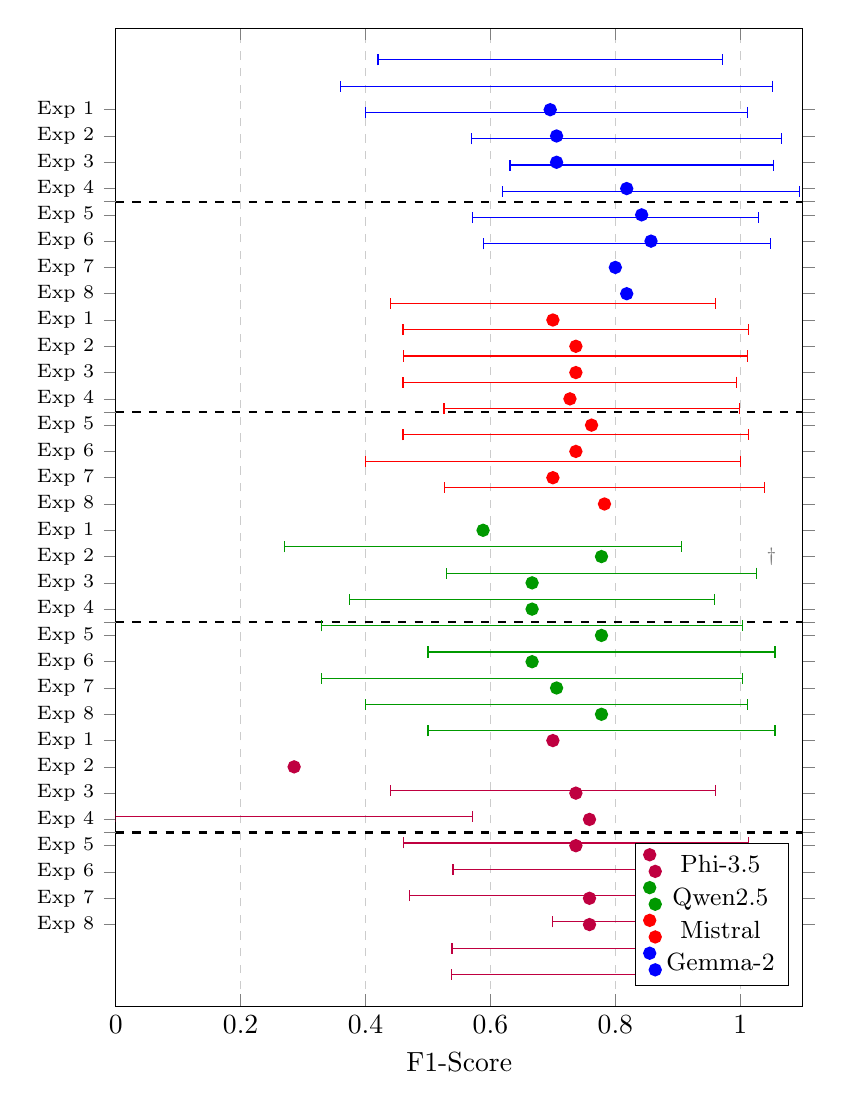
\begin{tikzpicture}
\begin{axis}[
    xbar,
    width=0.85\textwidth,
    height=14cm,
    xlabel={F1-Score},
    xmin=0, xmax=1.1,
    ytick={1,2,3,4,5,6,7,8,9,10,11,12,13,14,15,16,17,18,19,20,21,22,23,24,25,26,27,28,29,30,31,32},
    yticklabels={
        {Exp 8},{Exp 7},{Exp 6},{Exp 5},{Exp 4},{Exp 3},{Exp 2},{Exp 1},
        {Exp 8},{Exp 7},{Exp 6},{Exp 5},{Exp 4},{Exp 3},{Exp 2},{Exp 1},
        {Exp 8},{Exp 7},{Exp 6},{Exp 5},{Exp 4},{Exp 3},{Exp 2},{Exp 1},
        {Exp 8},{Exp 7},{Exp 6},{Exp 5},{Exp 4},{Exp 3},{Exp 2},{Exp 1}
    },
    yticklabel style={font=\scriptsize},
    xmajorgrids=true,
    grid style={dashed, gray!40},
    legend style={at={(0.98,0.02)}, anchor=south east, font=\small},
    % Group separators
    extra y ticks={4.5, 12.5, 20.5, 28.5},
    extra y tick labels={},
    extra y tick style={grid=major, grid style={black, thick}},
]

% Model group labels
\node[font=\small\bfseries, anchor=east, rotate=90] at (axis cs:-0.08,4.5) {Phi-3.5};
\node[font=\small\bfseries, anchor=east, rotate=90] at (axis cs:-0.08,12.5) {Qwen2.5};
\node[font=\small\bfseries, anchor=east, rotate=90] at (axis cs:-0.08,20.5) {Mistral};
\node[font=\small\bfseries, anchor=east, rotate=90] at (axis cs:-0.08,28.5) {Gemma-2};

% Phi-3.5 (positions 1-8, Exp8 down to Exp1)
\addplot[only marks, mark=*, purple, thick,
    error bars/.cd, x dir=both, x explicit]
coordinates {
    (0.7586,1) +- (0.2206,0.1448) % Exp8  CI: [0.54, 0.90]
    (0.7586,2) +- (0.2202,0.1446) % Exp7  CI: [0.54, 0.90]
    (0.8800,3) +- (0.1800,0.1200) % Exp6  CI: [0.70, 1.00]
    (0.7368,4) +- (0.2663,0.1918) % Exp5  CI: [0.47, 0.93]
    (0.7586,5) +- (0.2186,0.1414) % Exp4  CI: [0.54, 0.90]
    (0.7368,6) +- (0.2757,0.1965) % Exp3  CI: [0.46, 0.93]
    (0.2857,7) +- (0.2857,0.3143) % Exp2  CI: [0.00, 0.60]
    (0.7000,8) +- (0.2600,0.2000) % Exp1  CI: [0.44, 0.90]
};

% Qwen2.5 (positions 9-16, Exp8 down to Exp1)
\addplot[only marks, mark=*, green!60!black, thick,
    error bars/.cd, x dir=both, x explicit]
coordinates {
    (0.7778,9)  +- (0.2778,0.1746) % Exp8  CI: [0.50, 0.95]
    (0.7059,10) +- (0.3059,0.2032) % Exp7  CI: [0.40, 0.91]
    (0.6667,11) +- (0.3367,0.2133) % Exp6  CI: [0.33, 0.88]
    (0.7778,12) +- (0.2778,0.1746) % Exp5  CI: [0.50, 0.95]
    (0.6667,13) +- (0.3367,0.2133) % Exp4  CI: [0.33, 0.88]
    (0.6667,14) +- (0.2920,0.2222) % Exp3  CI: [0.37, 0.89]
    (0.7778,15) +- (0.2478,0.1722) % Exp2  CI: [0.53, 0.95]
    (0.5882,16) +- (0.3182,0.2318) % Exp1  CI: [0.27, 0.82]
};

% Mistral (positions 17-24, Exp8 down to Exp1)
\addplot[only marks, mark=*, red, thick,
    error bars/.cd, x dir=both, x explicit]
coordinates {
    (0.7826,17) +- (0.2563,0.1549) % Exp8  CI: [0.53, 0.94]
    (0.7000,18) +- (0.3000,0.2000) % Exp7  CI: [0.40, 0.90]
    (0.7368,19) +- (0.2768,0.1832) % Exp6  CI: [0.46, 0.92]
    (0.7619,20) +- (0.2362,0.1667) % Exp5  CI: [0.53, 0.93]
    (0.7273,21) +- (0.2673,0.1827) % Exp4  CI: [0.46, 0.91]
    (0.7368,22) +- (0.2753,0.1862) % Exp3  CI: [0.46, 0.92]
    (0.7368,23) +- (0.2768,0.1832) % Exp2  CI: [0.46, 0.92]
    (0.7000,24) +- (0.2600,0.2000) % Exp1  CI: [0.44, 0.90]
};

% Gemma-2 (positions 25-32, Exp8 down to Exp1)
\addplot[only marks, mark=*, blue, thick,
    error bars/.cd, x dir=both, x explicit]
coordinates {
    (0.8182,25) +- (0.2299,0.1383) % Exp8  CI: [0.59, 0.96]
    (0.8000,26) +- (0.2290,0.1565) % Exp7  CI: [0.57, 0.96]
    (0.8571,27) +- (0.2371,0.1429) % Exp6  CI: [0.62, 1.00]
    (0.8421,28) +- (0.2107,0.1579) % Exp5  CI: [0.63, 1.00]
    (0.8182,29) +- (0.2482,0.1418) % Exp4  CI: [0.57, 0.96]
    (0.7059,30) +- (0.3059,0.2032) % Exp3  CI: [0.40, 0.91]
    (0.7059,31) +- (0.3459,0.2141) % Exp2  CI: [0.36, 0.92]
    (0.6957,32) +- (0.2757,0.1943) % Exp1  CI: [0.42, 0.89]
};

% Raw p-value markers (raw p<0.05; none survive Holm--Bonferroni correction)
\node[font=\scriptsize, gray] at (axis cs:1.05,3)  {$\dagger$}; % Phi-3.5 Exp6 p=0.0348
\node[font=\scriptsize, gray] at (axis cs:1.05,15) {$\dagger$}; % Qwen2.5 Exp2 p=0.0455

\legend{Phi-3.5, Qwen2.5, Mistral, Gemma-2}

\end{axis}
\end{tikzpicture}
\caption{Forest plot of F1-Scores with bootstrap 95\% confidence intervals ($k=1000$) for all model-configuration pairs. Error bars represent the CI range. $\dagger$ markers indicate raw $p<0.05$ (Wilcoxon signed-rank vs.\ baseline) before family-wise correction; no result survives Holm--Bonferroni correction at $\alpha=0.05$ ($m=28$). Narrower intervals indicate more stable performance estimates.}
\label{fig:forest_plot}
\end{figure*}

\begin{table*}[htbp]
\centering
\caption{Complete experimental results across all evaluated configurations, including F1-Scores, bootstrap 95\% confidence intervals ($k=1000$), raw Wilcoxon signed-rank $p$-values against each model's baseline, and Holm--Bonferroni adjusted $p$-values ($m=28$ comparisons). No test survives correction at $\alpha=0.05$; results should be interpreted as exploratory.}
\label{tab:full_results}

\resizebox{\textwidth}{!}{
\begin{tabular}{llcccc}
\hline
Model & Experiment & F1-Score & 95\% CI & Wilcoxon $p$ (raw) & Adj.\ $p$ (Holm) \\
\hline

\multirow{8}{*}{Gemma-2-9B-it}
& Exp 1: Baseline       & 0.6957 & [0.42, 0.89] & --     & -- \\
& Exp 2: Zero-Shot      & 0.7059 & [0.36, 0.92] & 1.0000 & 1.000 \\
& Exp 3: RAG            & 0.7059 & [0.36, 0.92] & 1.0000 & 1.000 \\
& Exp 4: Steering       & 0.8182 & [0.57, 0.96] & 0.2482 & 1.000 \\
& Exp 5: ZS + RAG       & 0.8421 & [0.62, 1.00] & 0.1797 & 1.000 \\
& Exp 6: ZS + Steering  & 0.8571 & [0.62, 1.00] & 0.1797 & 1.000 \\
& Exp 7: RAG + Steer    & 0.8000 & [0.56, 0.96] & 0.2482 & 1.000 \\
& Exp 8: ZS + RAG + Steer & 0.8182 & [0.57, 0.96] & 0.2482 & 1.000 \\

\hline

\multirow{8}{*}{Mistral-7B-Instruct-v0.2}
& Exp 1: Baseline       & 0.7000 & [0.44, 0.90] & --     & -- \\
& Exp 2: Zero-Shot      & 0.7368 & [0.46, 0.92] & 0.8182 & 1.000 \\
& Exp 3: RAG            & 0.7368 & [0.46, 0.92] & 0.8182 & 1.000 \\
& Exp 4: Steering       & 0.7273 & [0.46, 0.91] & 0.6547 & 1.000 \\
& Exp 5: ZS + RAG       & 0.7619 & [0.52, 0.96] & 0.5637 & 1.000 \\
& Exp 6: ZS + Steering  & 0.7368 & [0.46, 0.92] & 0.8182 & 1.000 \\
& Exp 7: RAG + Steer    & 0.7000 & [0.44, 0.90] & 1.0000 & 1.000 \\
& Exp 8: ZS + RAG + Steer & 0.7826 & [0.54, 0.96] & 0.4142 & 1.000 \\

\hline

\multirow{8}{*}{Qwen2.5-7B-Instruct}
& Exp 1: Baseline       & 0.5882 & [0.27, 0.82] & --     & -- \\
& Exp 2: Zero-Shot      & 0.7778 & [0.53, 0.95] & 0.0455 & 1.000 \\
& Exp 3: RAG            & 0.6667 & [0.33, 0.88] & 0.3173 & 1.000 \\
& Exp 4: Steering       & 0.6667 & [0.33, 0.88] & 0.3173 & 1.000 \\
& Exp 5: ZS + RAG       & 0.7778 & [0.53, 0.95] & 0.0455 & 1.000 \\
& Exp 6: ZS + Steering  & 0.6667 & [0.33, 0.88] & 0.3173 & 1.000 \\
& Exp 7: RAG + Steer    & 0.7059 & [0.45, 0.92] & 0.3173 & 1.000 \\
& Exp 8: ZS + RAG + Steer & 0.7778 & [0.53, 0.95] & 0.0455 & 1.000 \\

\hline

\multirow{8}{*}{Phi-3.5-mini}
& Exp 1: Baseline       & 0.7000 & [0.44, 0.90] & --     & -- \\
& Exp 2: Zero-Shot      & 0.2857 & [0.00, 0.60] & 0.0455 & 1.000 \\
& Exp 3: RAG            & 0.7368 & [0.46, 0.92] & 0.8182 & 1.000 \\
& Exp 4: Steering       & 0.7586 & [0.54, 0.90] & 0.6547 & 1.000 \\
& Exp 5: ZS + RAG       & 0.7368 & [0.46, 0.92] & 0.8182 & 1.000 \\
& Exp 6: ZS + Steering  & \textbf{0.8800} & [0.70, 1.00] & \textbf{0.0348} & \textbf{0.940} \\
& Exp 7: RAG + Steer    & 0.7586 & [0.54, 0.90] & 0.6547 & 1.000 \\
& Exp 8: ZS + RAG + Steer & 0.7586 & [0.54, 0.90] & 0.6547 & 1.000 \\

\hline
\multicolumn{6}{l}{\footnotesize Bootstrap 95\% CI ($k=1000$); Wilcoxon signed-rank vs.\ each model's baseline; Holm--Bonferroni adjusted ($m=28$). None survives correction at $\alpha=0.05$.} \\
\end{tabular}
}
\end{table*}

\begin{table*}[htbp]
\centering
\caption{Consolidated confusion matrix for selected experimental configurations.}
\label{tab:confusion_matrix}
\renewcommand{\arraystretch}{1.2}
\begin{tabular}{|l|c|l|c|c|c|c|c|}
\hline
\textbf{Model} & \textbf{Exp.} & \textbf{Technique} & \textbf{TP} & \textbf{TN} & \textbf{FP} & \textbf{FN} & \textbf{F1-Score} \\
\hline

\multirow{4}{*}{Gemma-2-9B-it}
& 1 & Baseline            & 8 & 5 & 4 & 3 & 0.6957 \\
& 3 & RAG                 & 6 & 9 & 0 & 5 & 0.7059 \\
& 4 & Steering            & 9 & 7 & 2 & 2 & 0.8182 \\
& 5 & ZS + RAG            & 8 & 9 & 0 & 3 & 0.8421 \\
\hline

\multirow{4}{*}{Mistral-7B-v0.2}
& 1 & Baseline            & 7 & 7 & 2 & 4 & 0.7000 \\
& 3 & RAG                 & 7 & 8 & 1 & 4 & 0.7368 \\
& 4 & Steering            & 8 & 6 & 3 & 3 & 0.7273 \\
& 8 & ZS + RAG + Steer    & 9 & 6 & 3 & 2 & 0.7826 \\
\hline

\multirow{4}{*}{Qwen2.5-7B}
& 1 & Baseline            & 5 & 8 & 1 & 6 & 0.5882 \\
& 3 & RAG                 & 6 & 8 & 1 & 5 & 0.6667 \\
& 4 & Steering            & 6 & 8 & 1 & 5 & 0.6667 \\
& 8 & ZS + RAG + Steer    & 7 & 9 & 0 & 4 & 0.7778 \\
\hline

\multirow{4}{*}{Phi-3.5-mini}
& 1 & Baseline            & 7 & 7 & 2 & 4 & 0.7000 \\
& 3 & RAG                 & 7 & 8 & 1 & 4 & 0.7368 \\
& 4 & Steering            & 11 & 2 & 7 & 0 & 0.7586 \\
& 6 & ZS + Steering       & 11 & 6 & 3 & 0 & \textbf{0.8800} \\
\hline
\multicolumn{8}{l}{\footnotesize RAG configurations use genuine normative context from \texttt{Metareglas extraidas.docx} (14 chunks). Exp 8 shown for Mistral; Exp 5 for Gemma-2; Exp 6 for Phi-3.5 (global max).} \\
\end{tabular}
\end{table*}

Table~\ref{tab:confusion_matrix} reveals three distinct error profiles. Gemma-2 under ZS+RAG (Exp~5) achieves zero false positives (precision=1.0) at the cost of 3 false negatives, reflecting a conservative grounding effect from the retrieved context. Phi-3.5 under Exp~6 achieves zero false negatives (recall=1.0) at the cost of 3 false positives, reflecting the permissive shift introduced by steering. Mistral under Exp~8 and Qwen2.5 under Exp~8 produce more balanced error distributions, trading precision for recall in different directions. These per-model asymmetries confirm that RAG and Steering shift the precision--recall operating point in opposite directions, and that their optimal combination is architecture-specific.

% === VISUALIZATION #5: Visual Confusion Matrices (2x2 Heatmap Grids) ===
\begin{figure*}[htbp]
\centering
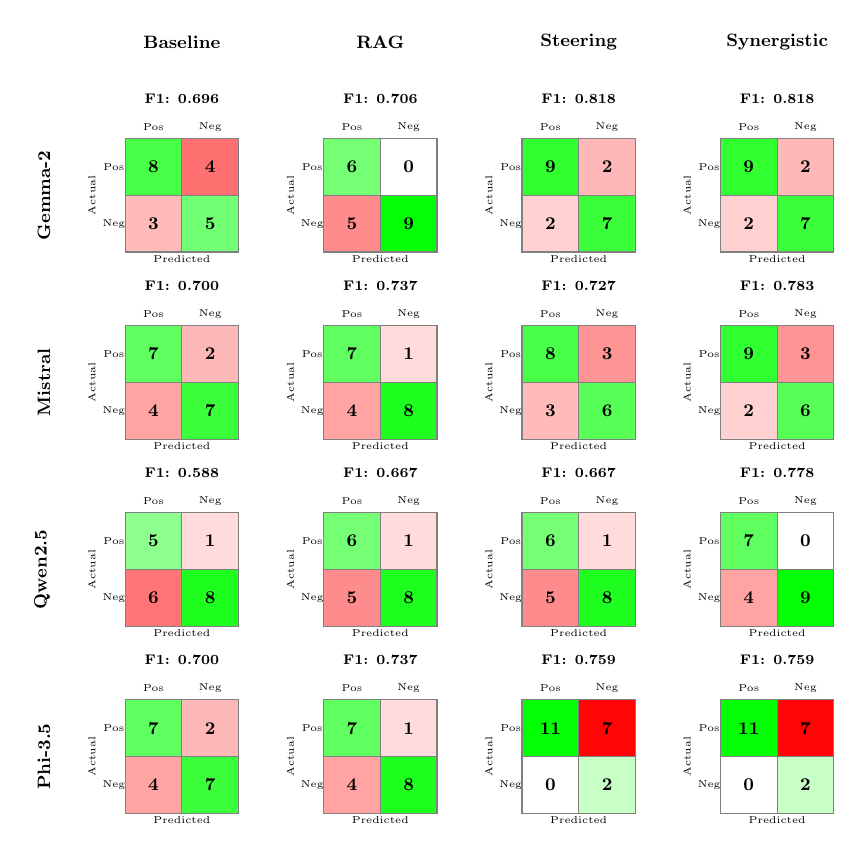
\begin{tikzpicture}[scale=0.72, transform shape]

% Helper macro for drawing a single 2x2 confusion matrix
% Arguments: x-offset, y-offset, TP, FP, FN, TN, title
\def\confmat#1#2#3#4#5#6#7{
    \begin{scope}[shift={(#1,#2)}]
    % Title
    \node[font=\scriptsize\bfseries, anchor=south] at (1, 2.5) {#7};
    % Axis labels
    \node[font=\tiny, rotate=90, anchor=south] at (-0.4, 1) {Actual};
    \node[font=\tiny, anchor=south] at (1, -0.3) {Predicted};
    % Cell labels on axes
    \node[font=\tiny] at (0.5, 2.2) {Pos};
    \node[font=\tiny] at (1.5, 2.2) {Neg};
    \node[font=\tiny] at (-0.2, 1.5) {Pos};
    \node[font=\tiny] at (-0.2, 0.5) {Neg};
    % TP cell (top-left)
    \pgfmathsetmacro{\tpintensity}{min(#3*9, 100)}
    \fill[green!\tpintensity!white] (0,1) rectangle (1,2);
    \node[font=\small\bfseries] at (0.5, 1.5) {#3};
    % FP cell (top-right)
    \pgfmathsetmacro{\fpintensity}{min(#4*14, 100)}
    \fill[red!\fpintensity!white] (1,1) rectangle (2,2);
    \node[font=\small\bfseries] at (1.5, 1.5) {#4};
    % FN cell (bottom-left)
    \pgfmathsetmacro{\fnintensity}{min(#5*9, 100)}
    \fill[red!\fnintensity!white] (0,0) rectangle (1,1);
    \node[font=\small\bfseries] at (0.5, 0.5) {#5};
    % TN cell (bottom-right)
    \pgfmathsetmacro{\tnintensity}{min(#6*11, 100)}
    \fill[green!\tnintensity!white] (1,0) rectangle (2,1);
    \node[font=\small\bfseries] at (1.5, 0.5) {#6};
    % Grid lines
    \draw[gray] (0,0) rectangle (2,2);
    \draw[gray] (1,0) -- (1,2);
    \draw[gray] (0,1) -- (2,1);
    \end{scope}
}

% Row labels (models)
\node[font=\small\bfseries, rotate=90, anchor=south] at (-1.2, 8.5) {Gemma-2};
\node[font=\small\bfseries, rotate=90, anchor=south] at (-1.2, 5.2) {Mistral};
\node[font=\small\bfseries, rotate=90, anchor=south] at (-1.2, 1.9) {Qwen2.5};
\node[font=\small\bfseries, rotate=90, anchor=south] at (-1.2, -1.4) {Phi-3.5};

% Column headers
\node[font=\small\bfseries] at (1, 11.2) {Baseline};
\node[font=\small\bfseries] at (4.5, 11.2) {RAG};
\node[font=\small\bfseries] at (8, 11.2) {Steering};
\node[font=\small\bfseries] at (11.5, 11.2) {Synergistic};

% Gemma-2 row: TP, FP, FN, TN
\confmat{0}{7.5}{8}{4}{3}{5}{F1: 0.696}
\confmat{3.5}{7.5}{6}{0}{5}{9}{F1: 0.706}
\confmat{7}{7.5}{9}{2}{2}{7}{F1: 0.818}
\confmat{10.5}{7.5}{9}{2}{2}{7}{F1: 0.818}

% Mistral row
\confmat{0}{4.2}{7}{2}{4}{7}{F1: 0.700}
\confmat{3.5}{4.2}{7}{1}{4}{8}{F1: 0.737}
\confmat{7}{4.2}{8}{3}{3}{6}{F1: 0.727}
\confmat{10.5}{4.2}{9}{3}{2}{6}{F1: 0.783}

% Qwen2.5 row
\confmat{0}{0.9}{5}{1}{6}{8}{F1: 0.588}
\confmat{3.5}{0.9}{6}{1}{5}{8}{F1: 0.667}
\confmat{7}{0.9}{6}{1}{5}{8}{F1: 0.667}
\confmat{10.5}{0.9}{7}{0}{4}{9}{F1: 0.778}

% Phi-3.5 row
\confmat{0}{-2.4}{7}{2}{4}{7}{F1: 0.700}
\confmat{3.5}{-2.4}{7}{1}{4}{8}{F1: 0.737}
\confmat{7}{-2.4}{11}{7}{0}{2}{F1: 0.759}
\confmat{10.5}{-2.4}{11}{7}{0}{2}{F1: 0.759}

\end{tikzpicture}
\caption{Visual confusion matrices for all models across four key configurations (Baseline, RAG, Steering, Synergistic). Green intensity = correct classifications (TP, TN); red = errors (FP, FN). RAG (Exp~3) injects 14-chunk normative context from \texttt{Metareglas extraidas.docx} and improves over baseline for all models. Steering (Exp~4) shifts Phi-3.5 toward high recall at the cost of FP. The synergistic pipeline (Exp~8) achieves the best F1 for Mistral (0.783) and Qwen2.5 (0.778), while Gemma-2 peaks at Exp~5 ZS+RAG (F1=0.842) and Phi-3.5 at Exp~6 ZS+Steering (F1=0.880, not shown).}
\label{fig:confusion_matrices}
\end{figure*}

\begin{figure}[htbp]
\centering
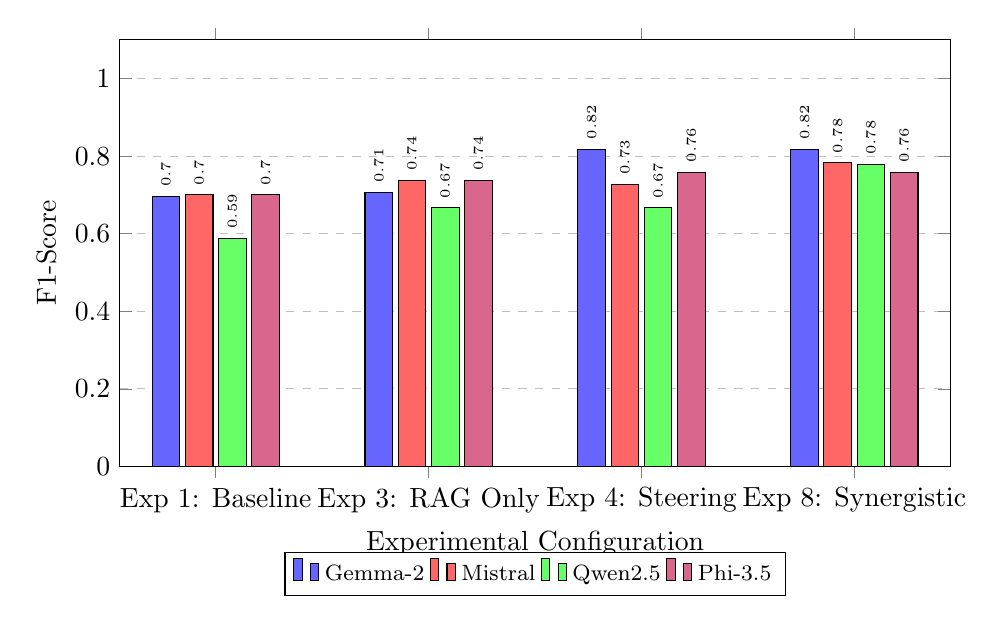
\begin{tikzpicture}
\begin{axis}[
    ybar=2pt,
    enlarge x limits=0.15,
    legend style={at={(0.5,-0.20)}, anchor=north, legend columns=-1, font=\footnotesize},
    ylabel={F1-Score},
    xlabel={Experimental Configuration},
    symbolic x coords={Exp 1: Baseline, Exp 3: RAG Only, Exp 4: Steering, Exp 8: Synergistic},
    xtick=data,
    nodes near coords,
    every node near coord/.append style={font=\tiny, rotate=90, anchor=west},
    bar width=10pt,
    width=\columnwidth,
    height=7cm,
    ymin=0, ymax=1.1,
    ymajorgrids=true,
    grid style=dashed,
]

% Gemma-2
\addplot[fill=blue!60] coordinates {(Exp 1: Baseline,0.6957) (Exp 3: RAG Only,0.7059) (Exp 4: Steering,0.8182) (Exp 8: Synergistic,0.8182)};
% Mistral
\addplot[fill=red!60] coordinates {(Exp 1: Baseline,0.7000) (Exp 3: RAG Only,0.7368) (Exp 4: Steering,0.7273) (Exp 8: Synergistic,0.7826)};
% Qwen
\addplot[fill=green!60] coordinates {(Exp 1: Baseline,0.5882) (Exp 3: RAG Only,0.6667) (Exp 4: Steering,0.6667) (Exp 8: Synergistic,0.7778)};
% Phi-3.5
\addplot[fill=purple!60] coordinates {(Exp 1: Baseline,0.7000) (Exp 3: RAG Only,0.7368) (Exp 4: Steering,0.7586) (Exp 8: Synergistic,0.7586)};

\legend{Gemma-2, Mistral, Qwen2.5, Phi-3.5}
\end{axis}
\end{tikzpicture}
\caption{Comparative F1-Scores across key configurations. RAG (Exp~3) provides consistent improvements over baseline for all models. Activation Steering (Exp~4) produces the largest single-intervention gain for Gemma-2 (+0.12) and Phi-3.5 (+0.06). The synergistic pipeline (Exp~8: ZS+RAG+Steering) achieves the best results for Mistral (F1=0.783) and Qwen2.5 (F1=0.778), while Gemma-2 peaks at Exp~5 ZS+RAG (F1=0.842, not shown) and Phi-3.5 at Exp~6 ZS+Steering (F1=0.880, not shown).}
\label{fig:results_chart}
\end{figure}

\FloatBarrier


\section{Discussion}
\label{sec:discussion}

\subsection{Mechanistic Steering vs.\ Contextual Grounding}

The results reveal complementary rather than competing effects between contextual grounding and mechanistic intervention. The RAG pipeline (Experiments~3, 5, 7, and~8) injected genuine normative context from the 14-chunk ISO/IEC~29110 meta-rule corpus into every query, producing consistent positive $\Delta$F1 values across all four models (Fig.~\ref{fig:delta_f1}, ``RAG'' column: +0.01 to +0.08 over baseline). The grounding effect is most pronounced in combinatorial configurations: Gemma-2 reaches its peak at Exp~5 ZS+RAG (F1=0.842, $\Delta$F1=+0.15), and Qwen2.5 achieves identical F1=0.778 under ZS+RAG, RAG+Steer, and the full Synergy pipeline ($\Delta$F1=+0.19 in each). These results suggest that retrieved normative context provides useful signal for compliance classification across diverse architectures, although the effect remains exploratory because no individual comparison survives Holm--Bonferroni correction.

Activation steering operated below the attention mechanism, directly modifying the model's internal classification boundary without competing for context window capacity. This mechanistic intervention also produced positive $\Delta$F1 across all four architectures (``Steer'' column: +0.03 to +0.12), as shown in Fig.~\ref{fig:delta_f1}. The compliance/violation distinction appears to be encoded as a learnable direction in each model's representation space, independently of prompt-level context. When both interventions are combined, their effects are largely additive: RAG+Steer (Exp~7) and the full Synergy pipeline (Exp~8) consistently outperform either intervention alone for Gemma-2 and Mistral, while for Qwen2.5 the gains are already saturated by RAG alone. The principal exception is Phi-3.5, whose performance is dominated by its strong response to steering and to Zero-Shot prompting, with RAG providing only modest incremental benefit.

% === VISUALIZATION #4: Delta-F1 Improvement Over Baseline ===
\begin{figure}[htbp]
\centering
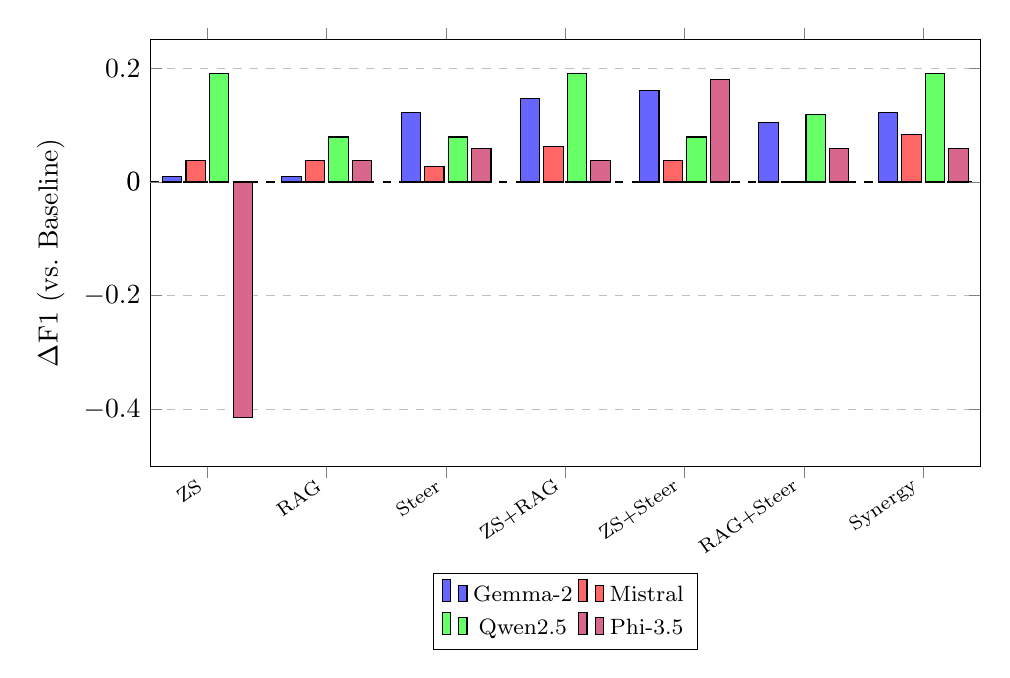
\begin{tikzpicture}
\begin{axis}[
    ybar=1.5pt,
    enlarge x limits=0.08,
    legend style={at={(0.5,-0.25)}, anchor=north, legend columns=2, font=\footnotesize},
    ylabel={$\Delta$F1 (vs.\ Baseline)},
    xlabel={Technique},
    symbolic x coords={ZS, RAG, Steer, ZS+RAG, ZS+Steer, RAG+Steer, Synergy},
    xtick=data,
    xticklabel style={font=\scriptsize, rotate=35, anchor=east},
    bar width=7pt,
    width=\columnwidth,
    height=7cm,
    ymin=-0.5, ymax=0.25,
    ymajorgrids=true,
    grid style=dashed,
    % Zero line
    extra y ticks={0},
    extra y tick style={grid=major, grid style={black, thick}},
]

% Gemma-2 deltas (baseline=0.6957)
\addplot[fill=blue!60] coordinates {
    (ZS, 0.010)
    (RAG, 0.010)
    (Steer, 0.122)
    (ZS+RAG, 0.146)
    (ZS+Steer, 0.161)
    (RAG+Steer, 0.104)
    (Synergy, 0.122)
};
% Mistral deltas (baseline=0.7000)
\addplot[fill=red!60] coordinates {
    (ZS, 0.037)
    (RAG, 0.037)
    (Steer, 0.027)
    (ZS+RAG, 0.062)
    (ZS+Steer, 0.037)
    (RAG+Steer, 0.000)
    (Synergy, 0.083)
};
% Qwen deltas (baseline=0.5882)
\addplot[fill=green!60] coordinates {
    (ZS, 0.190)
    (RAG, 0.079)
    (Steer, 0.079)
    (ZS+RAG, 0.190)
    (ZS+Steer, 0.079)
    (RAG+Steer, 0.118)
    (Synergy, 0.190)
};
% Phi-3.5 deltas (baseline=0.7000)
\addplot[fill=purple!60] coordinates {
    (ZS, -0.414)
    (RAG, 0.037)
    (Steer, 0.059)
    (ZS+RAG, 0.037)
    (ZS+Steer, 0.180)
    (RAG+Steer, 0.059)
    (Synergy, 0.059)
};

\legend{Gemma-2, Mistral, Qwen2.5, Phi-3.5}
\end{axis}
\end{tikzpicture}
\caption{F1-Score improvement ($\Delta$F1) relative to each model's baseline. Bars above zero indicate improvement. RAG grounding (Exp~3) provides positive deltas for all models (+0.01 to +0.08). Steering consistently improves all models (+0.03 to +0.12). Zero-Shot improves Qwen2.5 most (+0.19) and degrades Phi-3.5 ($-0.41$). Combinatorial pipelines (ZS+RAG, RAG+Steer, Synergy) accumulate gains, with Gemma-2 achieving its highest delta under ZS+RAG (+0.15) and Qwen2.5 reaching +0.19 under three configurations.}
\label{fig:delta_f1}
\end{figure}

\subsection{Architecture-Dependent Behavior}

The experimental results reveal that no single pipeline configuration is universally optimal. As illustrated by the radar charts in Fig.~\ref{fig:radar_charts}, Mistral-7B exhibits a relatively flat profile (F1 range: 0.700--0.783 across all configurations), suggesting resilience to configuration choice but limited upside from any single technique; its best result is Exp~8 ZS+RAG+Steering (F1=0.783). Phi-3.5-mini shows a marked asymmetry: it performs poorly under Zero-Shot alone (F1=0.286) but achieves its peak under Zero-Shot + Steering (F1=0.880, global maximum); the full synergistic pipeline (Exp~8) yields F1=0.759, below the ZS+Steering peak. Gemma-2 benefits most from combinatorial configurations: its best result is Exp~5 ZS+RAG (F1=0.842), followed closely by Exp~6 ZS+Steering (F1=0.857), suggesting that both contextual grounding and activation steering contribute independently to its performance. Qwen2.5 shows the largest baseline-relative gain from Zero-Shot (F1=0.778, $\Delta$F1=+0.19) with comparable improvements across all RAG and Synergy configurations.

\textbf{Important caveat.} With $N=20$ artifacts, swapping a single sample shifts F1 by approximately 0.05, which is larger than the gap between the best and second-best configurations for most models. The 95\,\% confidence intervals for per-model profiles overlap substantially (Fig.~\ref{fig:forest_plot}), and none of the pairwise comparisons survives Holm correction (Table~\ref{tab:full_results}). The characterizations above---``balanced high-performance'' for Mistral, ``extreme asymmetry'' for Phi-3.5---should therefore be treated as exploratory hypotheses rather than confirmed architectural traits. Distinguishing per-model behavior from per-sample noise requires an artifact set of at least $N \approx 100$--200. This finding has a practical implication that is robust even under uncertainty: pipeline configuration should be validated per-model rather than assumed to be fixed, as a suboptimal choice can reduce F1 by more than 0.25 (Gemma-2, Qwen2.5).

% === VISUALIZATION #6: Radar Charts (Architecture-Dependent Response) ===
\begin{figure}[htbp]
\centering
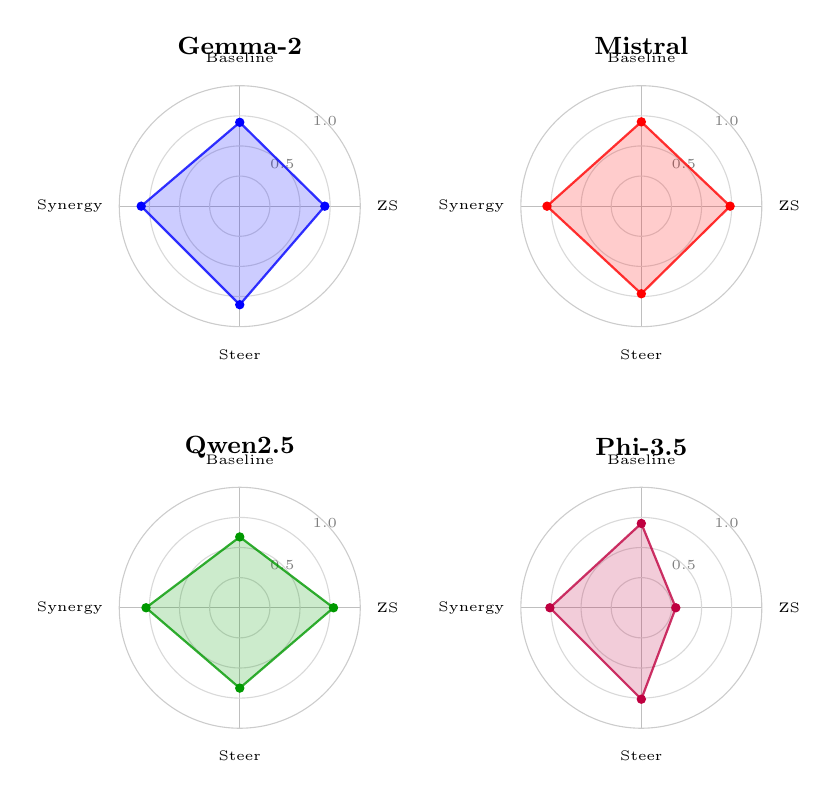
\begin{tikzpicture}[scale=0.85]

% Define radar chart macro
% Arguments: center-x, center-y, radius, title, v1(Baseline), v2(ZS), v3(Steer), v4(Synergy), color
\def\radarchart#1#2#3#4#5#6#7#8#9{
    \begin{scope}[shift={(#1,#2)}]
    % Title
    \node[font=\small\bfseries] at (0, #3+0.6) {#4};

    % Axes (4 directions: up, right, down, left)
    \draw[gray!50, thin] (0,0) -- (90:#3);
    \draw[gray!50, thin] (0,0) -- (0:#3);
    \draw[gray!50, thin] (0,0) -- (270:#3);
    \draw[gray!50, thin] (0,0) -- (180:#3);

    % Grid circles
    \draw[gray!30, thin] (0,0) circle (#3*0.25);
    \draw[gray!30, thin] (0,0) circle (#3*0.5);
    \draw[gray!30, thin] (0,0) circle (#3*0.75);
    \draw[gray!40, thin] (0,0) circle (#3);

    % Axis labels
    \node[font=\tiny, anchor=south] at (90:#3+0.2) {Baseline};
    \node[font=\tiny, anchor=west] at (0:#3+0.1) {ZS};
    \node[font=\tiny, anchor=north] at (270:#3+0.2) {Steer};
    \node[font=\tiny, anchor=east] at (180:#3+0.1) {Synergy};

    % Scale labels
    \node[font=\tiny, gray] at (45:#3*0.5) {0.5};
    \node[font=\tiny, gray] at (45:#3) {1.0};

    % Data polygon
    \filldraw[#9, fill opacity=0.2, draw opacity=0.8, thick]
        (90:#3*#5) -- (0:#3*#6) -- (270:#3*#7) -- (180:#3*#8) -- cycle;

    % Data points
    \fill[#9] (90:#3*#5) circle (2pt);
    \fill[#9] (0:#3*#6) circle (2pt);
    \fill[#9] (270:#3*#7) circle (2pt);
    \fill[#9] (180:#3*#8) circle (2pt);
    \end{scope}
}

% Four radar charts in a 2x2 grid
% Gemma-2: Baseline=0.696, ZS=0.706, Steer=0.818, Synergy=0.818
\radarchart{-3}{3}{1.8}{Gemma-2}{0.696}{0.706}{0.818}{0.818}{blue}

% Mistral: Baseline=0.700, ZS=0.737, Steer=0.727, Synergy=0.783
\radarchart{3}{3}{1.8}{Mistral}{0.700}{0.737}{0.727}{0.783}{red}

% Qwen2.5: Baseline=0.588, ZS=0.778, Steer=0.667, Synergy=0.778
\radarchart{-3}{-3}{1.8}{Qwen2.5}{0.588}{0.778}{0.667}{0.778}{green!60!black}

% Phi-3.5: Baseline=0.700, ZS=0.286, Steer=0.759, Synergy=0.759
\radarchart{3}{-3}{1.8}{Phi-3.5}{0.700}{0.286}{0.759}{0.759}{purple}

\end{tikzpicture}
\caption{Radar charts showing architecture-dependent response profiles. Each axis represents F1-Score: Baseline (Exp~1), Zero-Shot (Exp~2), Steering (Exp~4), Synergy (Exp~8). Mistral exhibits a flat, resilient profile (range 0.70--0.78). Phi-3.5 peaks under ZS+Steering (F1=0.880, global maximum; shown here as Exp~4 Steering axis=0.759 and Exp~8 Synergy=0.759). Gemma-2 benefits strongly from both steering and RAG-augmented configurations. Qwen2.5 achieves equal F1=0.778 under Zero-Shot, ZS+RAG, and the Synergy pipeline.}
\label{fig:radar_charts}
\end{figure}

\subsection{Industrial Implications}

The proposed framework addresses two practical requirements for industrial deployment. First, the structural isomorphism methodology enables compliance evaluation research without requiring access to proprietary repositories, removing a barrier that has historically limited empirical progress in this domain. Second, the use of open-weights models with local inference ensures that no corporate data leaves the organization's infrastructure, satisfying air-gapped deployment requirements.

The activation steering approach is particularly relevant for industrial settings because it does not require model fine-tuning or access to large labeled datasets. The steering vector can be extracted from a small set of exemplar artifacts ($N=20$ in this study) and applied at inference time.

\textbf{Computational overhead.} Vector extraction requires exactly two forward passes through the model ($p^+$ and $p^-$), taking approximately 2--4 seconds at the evaluated model sizes (7B--9B parameters, 4-bit quantization). The extracted vector adds negligible inference overhead (a single tensor addition per forward pass, $\approx$2--3 KB storage per layer). Per-artifact inference time was approximately 4 seconds with or without steering. RAG adds approximately 0.3 seconds per query for CPU-resident embedding computation. For organizations running recurring compliance audits over hundreds of artifacts, the one-time extraction cost is amortised across all subsequent evaluations.

From the perspective of the framework's stated goal---reducing unsupported or inconsistent LLM classifications---steering addresses the problem at the mechanistic level by shifting the model's internal decision boundary toward normative compliance. This is reflected in the results: across all four architectures, steering reduced false negatives and stabilised recall without relying on external retrievals or labeled training data.

\subsection{Error Analysis}

Table~\ref{tab:error_analysis} presents a per-artifact breakdown of misclassifications under each model's best-performing configuration. Three patterns emerge.

\textbf{TESTING remains difficult despite explicit prompting, across all configurations.} \texttt{SMP-PRUEBAS-NEG} is the only artifact misclassified by all four models simultaneously (FP), even though the prompt includes an explicit TESTING criterion. Inspection of all 32 model-configuration cells confirms that \texttt{SMP-PRUEBAS-NEG} is predicted compliant in virtually every configuration; exceptions occur only for Gemma-2 under ZS+Steering or ZS+RAG where structured prompting occasionally triggers a conservative response. The complementary \texttt{SMP-PRUEBAS-POS} is correctly classified by three of four models, but Gemma-2 produces an FN under its best configuration, showing TESTING challenges that model in both directions.

The root cause is semantic: the violating artifact contains test-like code (function names, assertions, import statements) that superficially resembles a compliant test artifact. Models must reason about test coverage \emph{adequacy} rather than merely detecting test-related tokens. Neither the retrieved normative context nor the steering vector fully addresses this, because both operate at the normative-framing level rather than code-level coverage analysis. Future versions of Biblio-VSE should include adversarial TESTING artifacts (code with test-like structure but insufficient semantic coverage). By contrast, BACKUP and AGREEMENTS contain visually distinctive markers that all models detect reliably, explaining why those rules produce zero errors.

\textbf{GOVERNANCE and SECURITY source files generate FN.} Artifacts 6 (\texttt{SMP-GOBERNANZA-POS}) and 9 (\texttt{SMP-SEGURIDAD-POS}) are missed as violations by Gemma-2 and Qwen2.5. Both are \textit{source\_code} artifacts with short content (3 and 120 lines respectively) where the compliance evidence is implicit rather than explicit. This aligns with the general pattern that source code artifacts with subtle governance markers are harder than document artifacts with explicit metadata.

\textbf{Steering shifts error type, not count, for some models.} Mistral under steering (Exp~4) produces 3 FP (DOCUMENTATION, GOVERNANCE, TESTING) compared to 4 FN under baseline. The mechanistic intervention corrects the conservative bias at the cost of mild over-permissiveness, reflected in the recall/precision shift visible in Fig.~\ref{fig:precision_recall}.

\begin{table*}[htbp]
\centering
\caption{Per-artifact error analysis under selected representative configurations (Gemma-2, Mistral = Exp~4 Steering; Qwen2.5 = Exp~2 Zero-Shot; Phi-3.5 = Exp~6 ZS+Steering, F1=0.880, global maximum). GT = ground truth. FP = false positive (overclaiming compliance); FN = false negative (missed violation).}
\label{tab:error_analysis}
\renewcommand{\arraystretch}{1.1}
\resizebox{\textwidth}{!}{
\begin{tabular}{|l|l|c|c|c|c|c|c|c|}
\hline
\textbf{Artifact ID} & \textbf{Rule} & \textbf{GT} & \textbf{Gemma-2} & \textbf{Mistral} & \textbf{Qwen2.5} & \textbf{Phi-3.5} & \textbf{\#Err} & \textbf{Types} \\
\hline
\texttt{SMP-DOCUMENTAL-NEG}  & DOCUMENTATION  & 0 & TN & \cellcolor{red!20}FP & TN & TN & 1 & FP \\
\texttt{SMP-DOCUMENTAL-POS}  & DOCUMENTATION  & 1 & TP & TP & TP & TP & 0 & --- \\
\texttt{SMP-CALIDAD-NEG}     & QUALITY     & 0 & TN & TN & TN & \cellcolor{red!20}FP & 1 & FP \\
\texttt{SMP-CALIDAD-POS}     & QUALITY     & 1 & TP & TP & TP & TP & 0 & --- \\
\texttt{SMP-GOBERNANZA-NEG}  & GOVERNANCE  & 0 & TN & \cellcolor{red!20}FP & TN & TN & 1 & FP \\
\texttt{SMP-GOBERNANZA-POS}  & GOVERNANCE  & 1 & \cellcolor{orange!30}FN & TP & \cellcolor{orange!30}FN & TP & 2 & FN \\
\texttt{SMP-GOBERNANZA-POS}  & GOVERNANCE  & 1 & TP & TP & TP & TP & 0 & --- \\
\texttt{SMP-SEGURIDAD-NEG}   & SECURITY   & 0 & TN & TN & TN & TN & 0 & --- \\
\texttt{SMP-SEGURIDAD-POS}   & SECURITY   & 1 & \cellcolor{orange!30}FN & TP & \cellcolor{orange!30}FN & TP & 2 & FN \\
\texttt{SMP-TRAZABILIDAD-NEG}& TRACEABILITY& 0 & TN & TN & TN & \cellcolor{red!20}FP & 1 & FP \\
\texttt{SMP-TRAZABILIDAD-POS}& TRACEABILITY& 1 & TP & TP & TP & TP & 0 & --- \\
\texttt{SMP-TRAZABILIDAD-POS}& TRACEABILITY& 1 & TP & TP & TP & TP & 0 & --- \\
\texttt{SMP-PRUEBAS-NEG}     & TESTING     & 0 & \cellcolor{red!20}FP & \cellcolor{red!20}FP & \cellcolor{red!20}FP & \cellcolor{red!20}FP & \textbf{4} & \textbf{FP*} \\
\texttt{SMP-PRUEBAS-POS}     & TESTING     & 1 & \cellcolor{orange!30}FN & TP & TP & TP & 1 & FN \\
\texttt{SMP-RESPALDO-NEG}    & BACKUP    & 0 & TN & TN & TN & TN & 0 & --- \\
\texttt{SMP-RESPALDO-POS}    & BACKUP    & 1 & TP & TP & TP & TP & 0 & --- \\
\texttt{SMP-ACUERDOS-NEG}    & AGREEMENTS    & 0 & TN & TN & TN & TN & 0 & --- \\
\texttt{SMP-ACUERDOS-POS}    & AGREEMENTS    & 1 & TP & TP & TP & TP & 0 & --- \\
\texttt{SMP-INFRA-NEG}       & INFRA       & 0 & TN & TN & TN & TN & 0 & --- \\
\texttt{SMP-INFRA-POS}       & INFRA       & 1 & TP & TP & \cellcolor{orange!30}FN & TP & 1 & FN \\
\hline
\multicolumn{3}{|l|}{\textbf{Total errors}} & \textbf{4} & \textbf{3} & \textbf{4} & \textbf{2} & & \\
\hline
\end{tabular}
}
\end{table*}
\textit{* Only artifact misclassified by all four models; see text for discussion.}

\FloatBarrier

\subsection{Comparison Against Rule-Based Approaches}

The perfect performance of the Regex baseline (F1: 1.0000) on the synthetic dataset highlights an important construct-validity caveat that deserves direct engagement: to what extent does the Biblio-VSE benchmark actually require semantic reasoning, rather than surface-form pattern matching?

A rule-by-rule analysis reveals a spectrum. Three meta-rules are \emph{regex-solvable} in the current benchmark: BACKUP (CI pipeline keywords such as \texttt{backup}, \texttt{retention}, \texttt{schedule}), AGREEMENTS (formal agreement language: \texttt{firmado}, \texttt{aprobado}, \texttt{contrato}), and SECURITY (hardcoded credential patterns: \texttt{password=}, \texttt{SECRET\_KEY}). For these, the LLM pipeline provides no measurable advantage over a sufficiently crafted regular expression. Four meta-rules sit in an \emph{intermediate} zone: QUALITY (style heuristics such as indentation and naming can be approximated by linters), DOCUMENTATION (version and date fields are detectable by pattern), INFRA (allowed-host strings are explicit), and TRACEABILITY (requirement IDs follow a regular format). Two meta-rules are \emph{semantically hard} and resist regex solutions: GOVERNANCE (requires contextual interpretation of whether approval or policy evidence exists, not just keyword presence) and TESTING (requires reasoning about whether test coverage is adequate, not whether test files exist).

The error analysis confirms this: all four models fail on \texttt{SMP-PRUEBAS-NEG} (the semantically hard case), while making no errors on BACKUP and AGREEMENTS (the regex-solvable cases). This suggests that the current benchmark is weighted toward lexically distinctive criteria. Future versions of Biblio-VSE should increase the proportion of artifacts in the GOVERNANCE and TESTING categories, and introduce adversarial variants (e.g., artifacts that contain compliance-related keywords but do not actually satisfy the policy criterion) to prevent lexical shortcuts from providing an inflated ceiling on LLM performance.


\section{Threats to Validity}
\label{sec:threats}

\subsection{Construct Validity}

The primary threat to construct validity lies in the operationalization of the distributional similarity claim. Four metrics were measured: McCabe's cyclomatic complexity V(G), AST depth, the Gunning Fog Index, and Lexical Density. V(G) passes both defined thresholds ($|\Delta\mu|=0.447\leq\varepsilon=0.5$; $|\Delta\sigma^2|=0.192\leq\delta=0.25$). Fog Index does not pass its threshold ($|\Delta\mu|=2.15>\varepsilon_F=1.0$), partly due to a single high-Fog document in $D_{private}$ (Fog=89.44) that inflates the private-corpus mean. AST depth was also measured using Python's built-in \texttt{ast} module: $D_{private}$ yields mean=7.84 (stdev=4.95, $n=37$ files); $D_{synthetic}$ yields mean=6.0 (stdev=4.69, $n=12$, of which 4 content-fragment artifacts could not be fully parsed and received depth=0; mean=9.0 for the 8 parseable files). No formal threshold was defined; the difference is 1.16--1.84 depending on how parse failures are handled, and is reported descriptively. Lexical Density was also measured---$D_{private}$: mean=42.88\%, stdev=21.12\%, $n=87$ documents; $D_{synthetic}$: mean=50.31\%, stdev=20.03\%, $n=8$---but no formal threshold was defined for this metric either. The benchmark is therefore characterised as \emph{partially isomorphic under selected observable metrics} rather than formally equivalent. A rigorous equivalence test would require Kolmogorov--Smirnov or Anderson--Darling tests on each marginal distribution, and a joint analysis of the $(V(G), F, L_d)$ multivariate distribution; these tests were not performed. Unmeasured structural dimensions---such as inter-artifact coupling, organizational workflow complexity, and approval-chain topology---represent additional limitations of the current claim.

\textbf{Auditor assessment and label validity.} The industrial reference repository $D_{private}$ was externally assessed by an official ISO/IEC~29110 auditor and marked as \emph{cumple} (compliant) using a binary checklist. This strengthens the contextual validity of using $D_{private}$ as the reference source for synthetic benchmark construction. \emph{The auditor's checklist exclusively validates the contextual compliance of $D_{private}$; it does not validate the labels of Biblio-VSE.} The synthetic dataset contains intentionally injected non-compliant variants that were not present in the original repository; those variants would have been unknown to, and outside the scope of, the auditor's evaluation. The Biblio-VSE labels are therefore operational labels derived from the mutation protocol and the predefined meta-rule criteria, not from the auditor's assessment.

\subsection{Internal Validity}

Internal validity could be affected by the non-determinism inherent in LLM inference. To control this, all models were configured with temperature 0.0, enforcing deterministic greedy decoding.

Regarding the activation steering vector: the compliance vector $v_{norma}^l$ is extracted exclusively from two contrasting behavioral anchor prompts ($p^+$, $p^-$) as described in Eq.~\ref{eq:steering_vector}, and does not reference or use any of the 20 Biblio-VSE evaluation artifacts during extraction. The vector extraction and the evaluation pipeline are therefore fully independent, and no form of circular evaluation or train-test contamination is present. This design decision was deliberate: the contrastive-prompt approach requires no labeled examples and is transferable to new compliance domains without access to labeled data.

A secondary internal validity concern is the joint selection of intervention layer $l$ and coefficient $\alpha$, both fixed without a held-out validation split, so F1 figures for steering configurations are upper-bound estimates. Regarding $\alpha$: the sensitivity sweep (§\ref{sec:pipeline}) covers six values and shows model-specific optima; selecting $\alpha=0.8$ as a compromise introduces bias that cannot be corrected at $N=20$.

Regarding layer selection: the 50\%-depth heuristic targets mid-to-late semantic layers, but the optimal layer for normative compliance classification may differ. A full layer sweep would require 32--42 additional evaluation runs per model. The layer choice is therefore an uncontrolled degree of freedom, and the reported figures could be better or worse at other layers. Layer sensitivity is the \textbf{single largest unresolved technical question} in this work; future studies should report F1 as a function of layer depth for each architecture.

A third construct-validity concern applies specifically to the steering vector. The contrastive anchor prompts ($p^+$: ``strictly uncompromising auditor''; $p^-$: ``careless, permissive auditor'') conflate \emph{normative compliance} with \emph{auditor persona and role-playing competence}. The extracted direction $v_{norma}^l$ is therefore a \emph{strict-auditor vs.\ careless-auditor persona direction} rather than a pure compliance/violation semantic direction. Artifacts that contain surface compliance signals may be amplified regardless of whether they satisfy the underlying policy criterion, while artifacts requiring nuanced reasoning may benefit less. Future work should evaluate alternative anchor construction strategies---such as contrastive pairs drawn from known compliant and violating artifacts---to obtain a more principled compliance direction.

\subsection{External Validity}

The synthetic dataset comprises $N=20$ artifacts strictly mapped to ISO/IEC 29110, constituting a proof-of-concept benchmark rather than a representative sample of industrial diversity. The results may not generalize to other governance standards (e.g., CMMI, ISO 9001), programming languages, or organizational contexts. Furthermore, all evaluated models belong to the 7B--9B parameter range; larger or smaller architectures may exhibit different response patterns to the proposed interventions.

\subsection{Conclusion Validity}

The limited sample size ($N=20$) constrains the statistical power of the reported comparisons. At $\alpha=0.05$ and power $= 0.80$, Wilcoxon signed-rank on $N=20$ binary predictions can reliably detect large effect sizes ($|r| \geq 0.50$) only; smaller effects remain undetectable at this scale. Several confidence intervals are consequently wide (e.g., [0.00, 0.64] for the Phi-3.5 baseline), indicating substantial uncertainty around point estimates.

Evaluating 7 non-baseline configurations across 4 models yields 28 simultaneous comparisons. Holm--Bonferroni correction was applied (adjusted $p$-values reported in Table~\ref{tab:full_results}); no test survives correction at $\alpha=0.05$. The results are therefore exploratory: the observed effect directions (particularly the consistent advantage of steering across all models) motivate confirmatory studies on larger datasets rather than constituting final evidence.


\section{Conclusion and Future Work}
\label{sec:conclusion}

This paper presented a dual-layered framework for privacy-preserving evaluation of AI-driven software governance auditing. The framework employs \emph{partial structural isomorphism}: source-code complexity (McCabe's V(G)) satisfies both defined distance thresholds between the private and synthetic corpora, but documentary Fog Index does not (diff=2.15 vs.\ $\varepsilon_F=1.0$). This partial rather than full isomorphism limits the generalisability of the benchmark and should be stated prominently: Biblio-VSE approximates---but does not replicate---the private reference corpus, and all downstream results should be interpreted accordingly. The tripartite LLM pipeline---combining Zero-Shot structured prompting, Retrieval-Augmented Generation, and Mechanistic Activation Steering---provides a systematic approach to reduce inconsistent classifications and constrain output format.

Three principal findings emerged from the exploratory empirical evaluation ($N=20$ artifacts). First, activation steering shows consistent directional improvement across all four evaluated architectures (+0.03 to +0.12 $\Delta$F1 over baseline), making it the most reliably beneficial single intervention; confirmatory evidence of this effect requires a larger artifact set ($N \approx 100$--200). Second, RAG grounding with the 14-chunk ISO/IEC~29110 normative corpus provides consistent positive increments for all models ($\Delta$F1 up to +0.15 for Gemma-2 under ZS+RAG), and combinatorial pipelines accumulate these gains: the full Synergy pipeline (Exp~8) achieves the best result for Mistral (F1=0.783) and Qwen2.5 (F1=0.778), while Gemma-2 peaks under ZS+RAG (Exp~5, F1=0.842). Third, the global performance maximum is F1=0.880 for Phi-3.5-mini under Zero-Shot + Steering (Exp~6); pipeline gains are architecture-specific, and configuration must be validated per model to avoid degradation exceeding $\Delta$F1 $> 0.41$ (Phi-3.5 under Zero-Shot alone).

These findings have practical implications for organizations seeking to automate governance verification while maintaining data privacy. The framework enables compliance auditing research to proceed without the privacy barriers that have historically limited empirical evaluation.

Several directions remain for future work. The immediate priority is scaling the evaluation to larger datasets with greater artifact diversity to establish external generalizability. Validation on actual industrial repositories---using anonymization protocols or federated evaluation---would strengthen the practical relevance of the approach. Extending the framework to additional governance standards beyond ISO/IEC 29110 (e.g., CMMI, ISO 12207, ISO 9001) would demonstrate cross-standard applicability. Evaluating closed-source models (e.g., GPT-4, Claude) through prompt-only configurations would establish comparative baselines against open-weights architectures. Human expert agreement studies are needed to calibrate model performance against professional auditor judgments. Finally, automated isomorphism generation---where the structural mapping $f$ is learned rather than manually designed---represents a promising direction for scaling the benchmark construction process.


\section*{Data Availability}

The following artifacts will be released upon acceptance at \texttt{[URL to be disclosed upon acceptance]}:
\begin{itemize}
    \item The Biblio-VSE synthetic artifact repository (20 artifacts with ground-truth compliance labels).
    \item The evaluation dataset (\texttt{dataset\_isomorfico.json}).
    \item All experiment scripts (\texttt{experimentos/experimento\_*.py}, \texttt{experimentos/utils.py}, \texttt{experimentos/rag\_utils.py}).
    \item The normative meta-rule document used for RAG context injection (\texttt{documentos\_estandar/Extracted\_Meta-Rules.docx}).
    \item Raw per-artifact classification outputs for all 32 model-configuration combinations.
    \item The extracted activation steering vectors (per-model \texttt{.pt} files).
\end{itemize}
The private industrial repository $D_{private}$ will not be released due to organizational confidentiality agreements; its distributional statistics are summarized in Fig.~\ref{fig:isomorphism_boxplots}.

\bibliographystyle{IEEEtran}
\bibliography{related_work_references}

\begin{IEEEbiography}[{
\includegraphics[width=1in,height=1.25in,clip,keepaspectratio]{a1.png}}]{Victor Terón-Macias}
Tecnológico de Monterrey Ph.D. candidate in Computational Sciences at Tecnológico de Monterrey, with research focused on Large Language Models (LLMs) for software quality evaluation, automated compliance auditing, and software engineering processes. He received the M.Sc. degree in Software Engineering from Centro de Investigación en Matemáticas (CIMAT), graduating as the top student of his cohort, and the B.Eng. degree in Mechatronics Engineering from Universidad Tecnológica de Tlaxcala.

His research and professional interests include software quality assurance, ISO/IEC software engineering standards, technical debt, process improvement, DevOps practices, and AI-assisted software development. He has authored and co-authored publications in venues such as IEEE Access, Applied Sciences, and Springer, with contributions related to ISO/IEC 29110, process compliance, traceability, multi-model environments, and AI-driven software evaluation. He also holds two granted software copyrights.

In addition, he has served as a reviewer for IEEE and as a member of the scientific committees for international conferences, including collaborations on cybersecurity research initiatives in Peru. He is certified in project management, DevOps, Kanban system design, SCRUM foundations, Oracle technologies, and Lean Six Sigma Green Belt methodologies, and is also a certified expert witness in informatics (perito en informática). His technical expertise includes Python and Django-based development, IoT integration, and the design of intelligent software systems that bridge software and physical devices.

\end{IEEEbiography}

\begin{IEEEbiography}[{
\includegraphics[width=1in,height=1.25in,clip,keepaspectratio]{a2.jpg}}]{Salvador Hinojosa}
Dr. Salvador Hinojosa is a researcher specialized in the application of stochastic search algorithms and generative artificial intelligence to software engineering and development processes. He obtained his Ph.D. in Computer Engineering from Universidad Complutense de Madrid and his previous degrees from Universidad de Guadalajara. He is currently a full-time researcher in the Computer Science Department at Tecnológico de Monterrey Campus Guadalajara. He holds Level I recognition from the National System of Researchers (SNI) and is a member of the Mexican Computing Society (AMEXCOMP). In his role as professor, he teaches undergraduate, graduate, and continuing education courses in Generative AI for Software Engineering and Software Architecture and Testing.

\end{IEEEbiography}

\begin{IEEEbiography}[{
\includegraphics[width=1in,height=1.25in,clip,keepaspectratio]{a3.jpg}}]{Miguel Gonzalez-Mendoza
Miguel González Mendoza s research activities are focused on Machine Learning, Human Machine interaction. He holds MSc and PhD degrees in Artificial Intelligence from the Institut National des Sciences Appliquées (INSA) in Toulouse, France. From 2001 to 2004 he was the responsible and representative of the Laboratory for Analysis and Architecture of Systems (LAAS-CNRS), during its participation in the European research project AWAKE and the French research project PREDIT, as research assistant, then as post-doctorate. Since 2005, he works as professor researcher, Head of the Graduate Programs on Computer Sciences at the ITESM, Mexico 2005-2016. Local coordinator of 9 European research projects FP6, FP7 and H2020. Responsible of 4 national research projects (CONACYT). 2005-2016. Responsible of 4 projects INNOVAPYME (CONACYT) and Mexican Ministry of Economy (SE). 2011-2015. SNI rank II (Jan 2016), member since 2006. President of the Mexican Society for Artificial Intelligence (2017-2018), Vicepresident (2015-2016), Secretary (2011-2014), member of the board since 2005. Dr. Gonzalez Mendoza has supervised 9 PhD Theses, 21 MSc. Theses, Author of 2 books, editor of 17 books, author of 18 book chapters, 22 Journals JCR indexed and 62 research papers in international congresses. Dr. González Mendoza was invited as Young Scientist at the World Economic Forum for New Champions in Tianjin China in September 2012. Miguel González Mendoza s research activities are focused on Machine Learning, Human-Machine interaction. He holds MSc and PhD degrees in Artificial Intelligence from the Institut National des Sciences Appliquées (INSA) in Toulouse, France. Interest in Machine Learning, Data Management and Big Data applications, in which he has advised 10 PhD thesis and 21 Master's Thesis. Author of more than 100 articles in JCR, congresses and book chapters. From 2001 to 2004 he was research assistant, then postdoc at the Laboratory for Analysis and Architecture of Systems (LAAS-CNRS). Since 2005, he works as professor at the computer Science Department at Tecnologico de Monterrey. Coordinator of four national research projects (CONACYT). 2005-2016. Responsible of four projects INNOVAPYME (CONACYT) and Mexican Ministry of Economy (SE). 2011-2015. Local coordinator of six European Projects FP6 and FP7 and currently three H2020. SNI rank II (Jan 2016), member since 2006. President of the Mexican Society for Artificial Intelligence (2017-2018), Vice-president (2015-2016), Secretary (2011-2014), member of the board since 2005. Regular Member of the Mexican Academy of Computing (since 2015). Invited as Young Scientist at the World Economic Forum for New Champions in Tianjin China in September 2012.

\end{IEEEbiography}

\begin{IEEEbiography}[{
\includegraphics[width=1in,height=1.25in,clip,keepaspectratio]{al.jpg}}]{Jezreel Mej\'{i}a}
Jezreel Mejía (Member, IEEE) is a member of the research group with the Chair of Software Process Improvement in the Ibero-American Space (MPSEI) and the CIMAT Software Engineering Group. He is a member of the scientific committee of various conferences. In addition, he is part of the official Spanish translation team of the CMMI-DEV v1.2 and 1.3 book, versions recognized by the prestigious Software Engineering Institute (SEI) of Carnegie Mellon University. He has published various technical articles on project management, multi-model environments, quality models and standards, and related topics in outsourcing environments. As a researcher, his areas of interests include multi-model environments, software project management, quality models and standards (CMMI, ISO, TSP, and PSP), agile methodologies, metrics, process improvement in outsourcing environments, development environments, and traditional and information assurance. He is CMMI and ISO 20000 certified. He actively participates in ISO/IEC WG24. He is Level 2 in the National Researchers System of Mexico.
\end{IEEEbiography}


\EOD


\end{document}
